\part{Results}
\label{pa:results}
\chapter{Ranklust as a tool for researchers}
\section{The planned workflow in general}
First off is the general workflow:
\begin{figure}
    \label{fig:ranklust-workflow}
    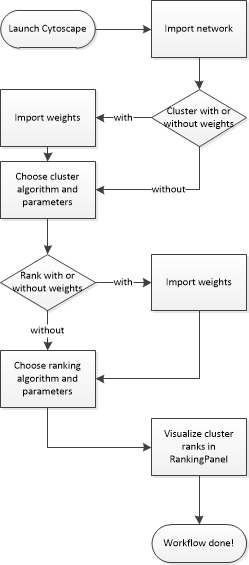
\includegraphics[scale=0.8]{ranklust_workflow}
\end{figure}

\section{Detailed walk-through of using Ranklust}
To go into more detail, here is the startup screen that the user is met with
after launching Cytoscape. This assumes that clusterMaker2 with the Ranklust
contribution is already installed into Cytoscape.
\begin{figure}
    \label{fig:startup}
    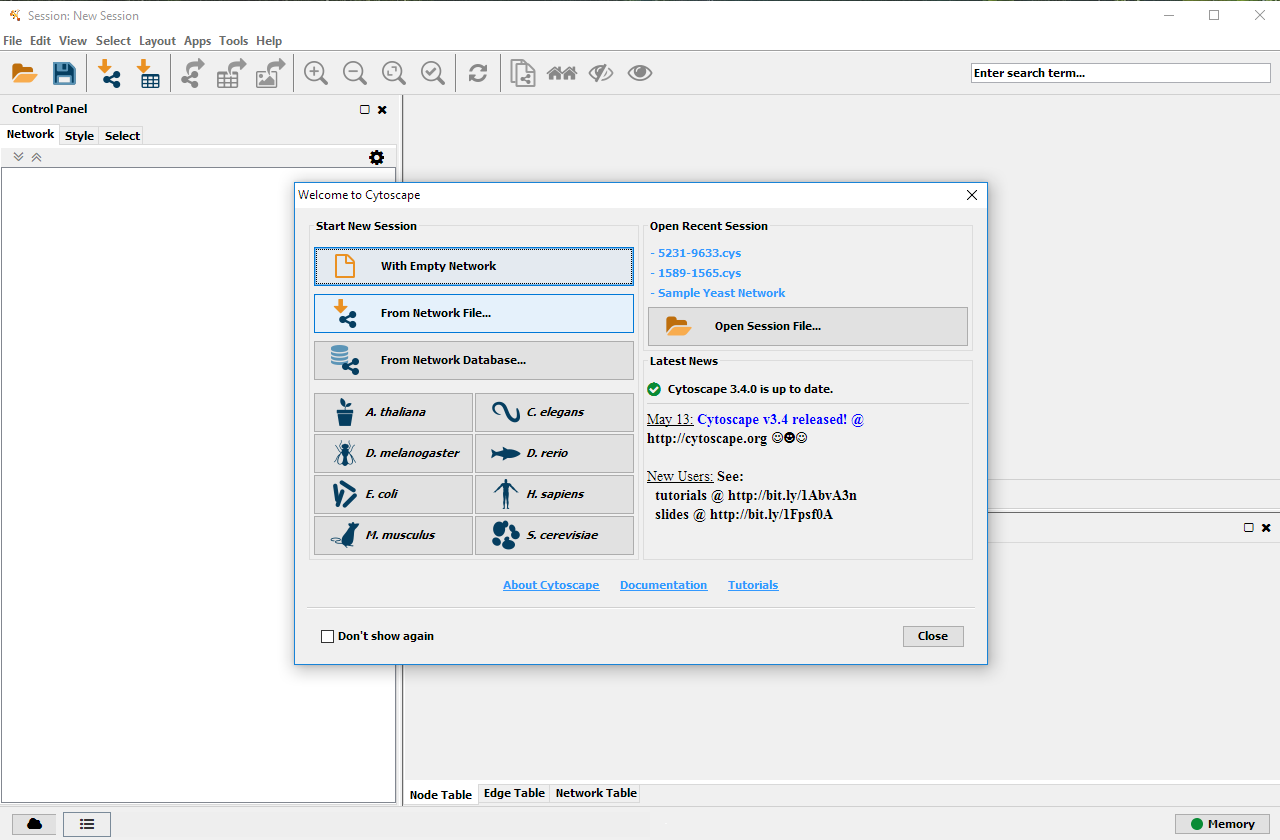
\includegraphics[width=15cm]{1-startup}
\end{figure}

This screen is what opens up after opting to import a network and choose a
network file consisting of a header that represents source and target node
columns, a\_alias and b\_alias.
\begin{figure}[H]
    \label{fig:import}
    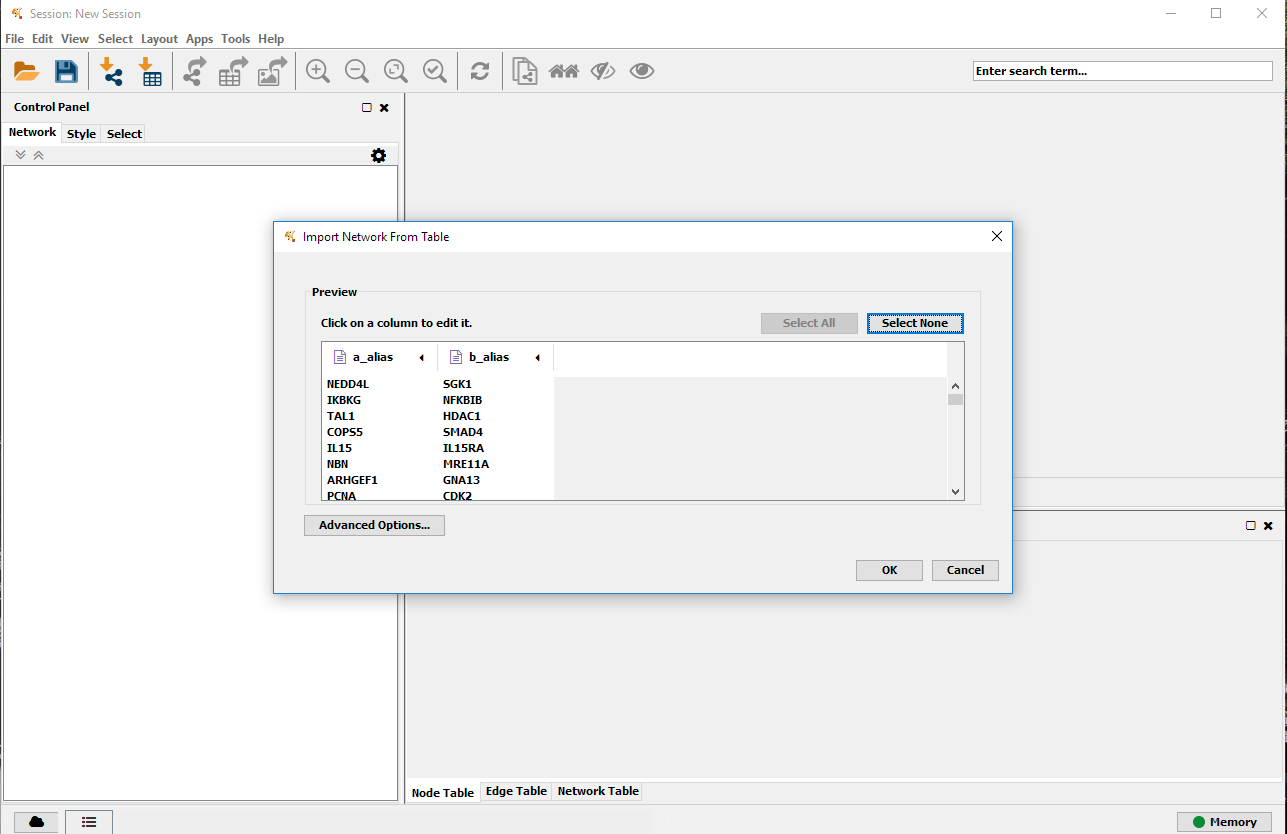
\includegraphics[width=15cm]{2-import}
\end{figure}

It is important to tell Cytoscape which column is considered as the source and
target column, as shown here. In this thesis, genes has been the primary key
identifier in both source and target column.
\begin{figure}[H]
    \label{fig:nodes}
    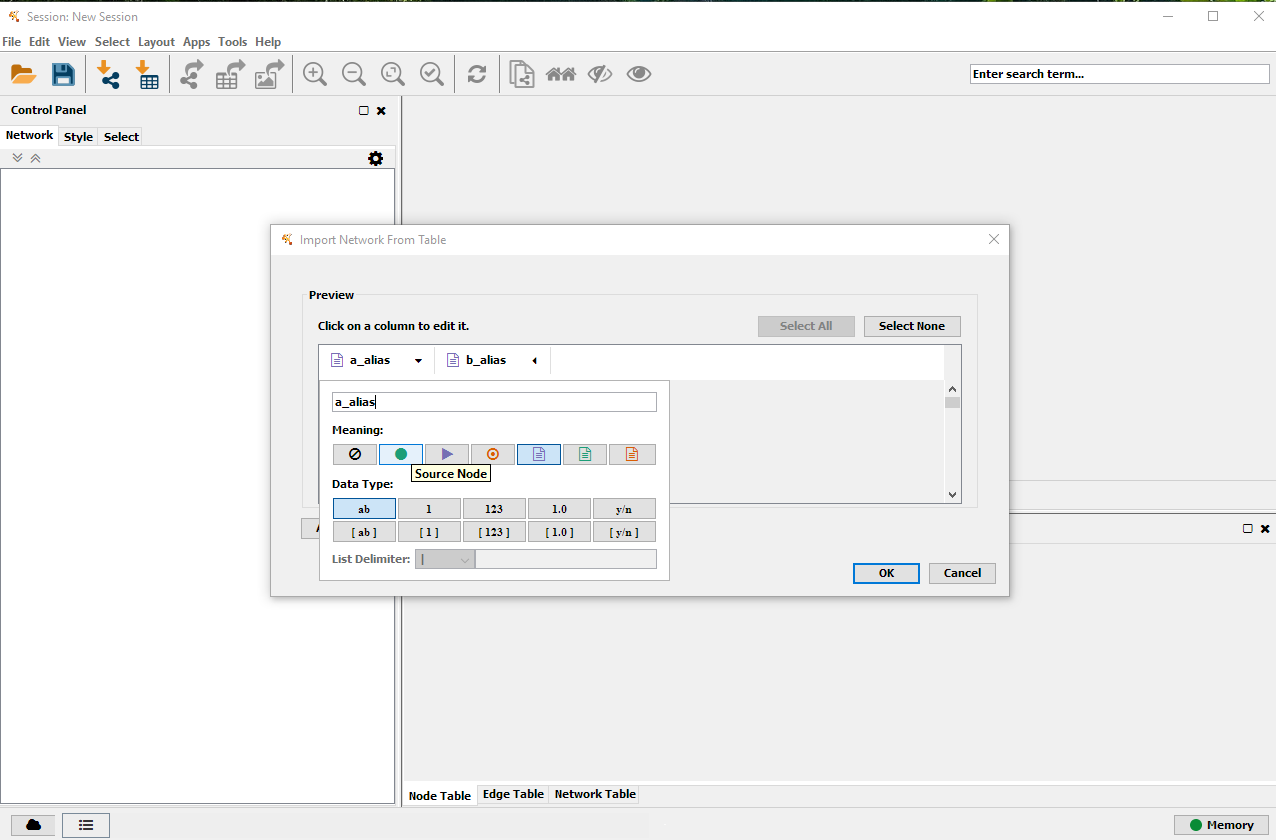
\includegraphics[width=15cm]{3-nodes}
\end{figure}

This is how Cytoscape looks after importing the network and it has finished its
standard style layout algorithm, which happens automatically after clicking "OK"
in the previous screen - having set everything to the correct settings.
\begin{figure}[H]
    \label{fig:imported-network}
    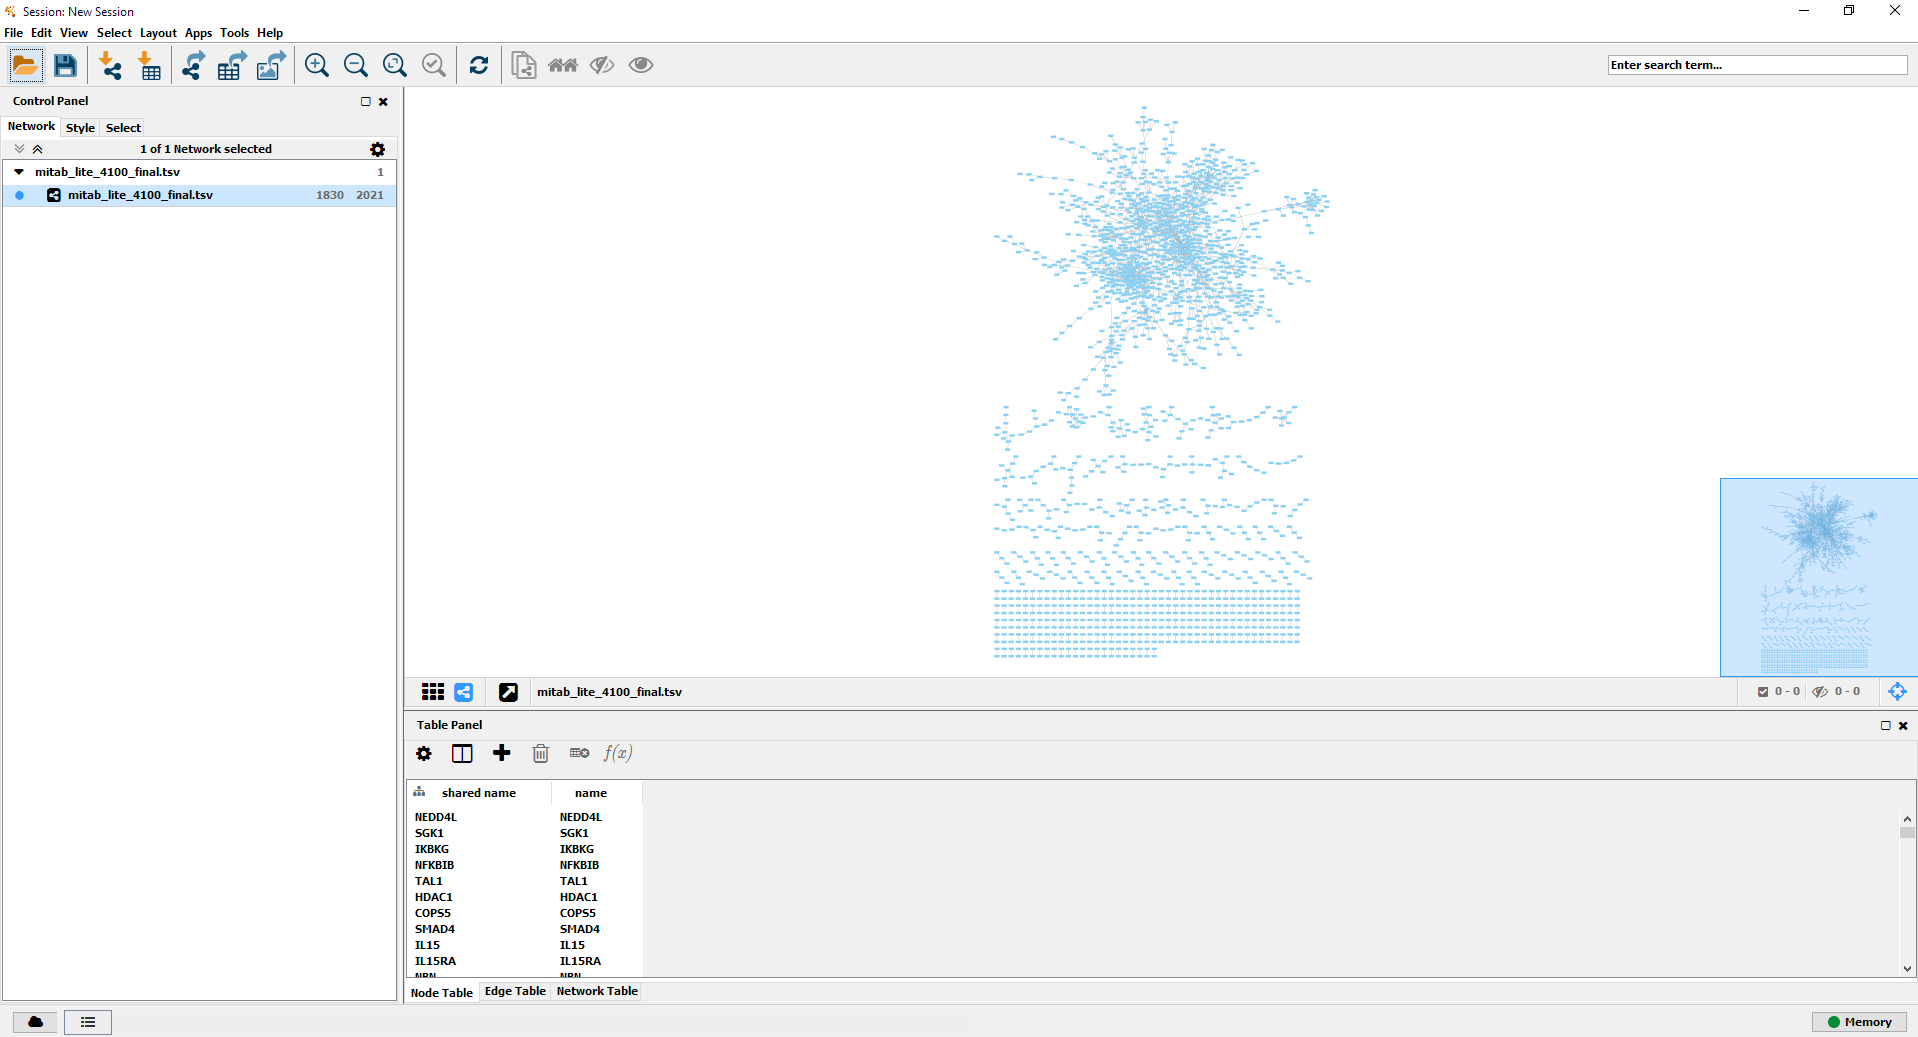
\includegraphics[width=15cm]{4-imported-network}
\end{figure}

If the user wishes to weight nodes for clustering or the ranking of them, it is
possible to do this with the "Import Columns From Table" function.
\begin{figure}[H]
    \label{fig:import-table}
    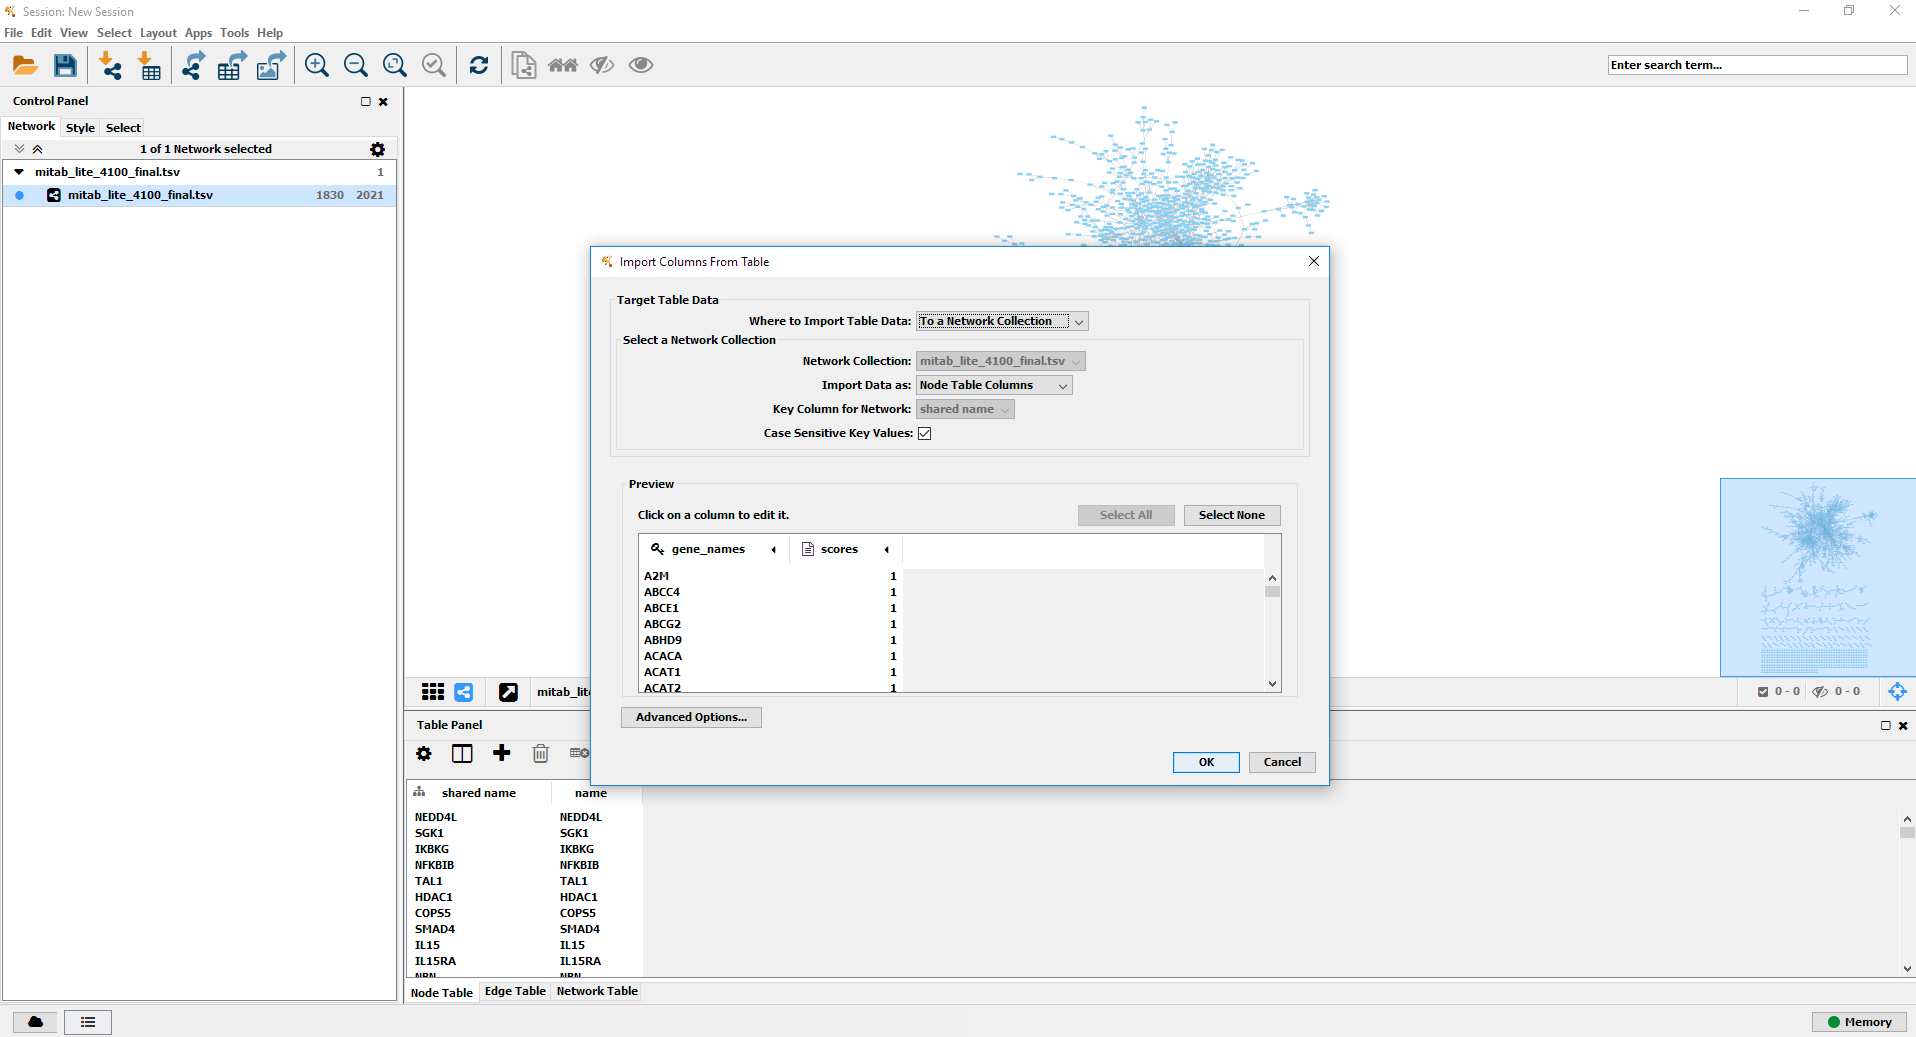
\includegraphics[width=15cm]{5-import-table}
\end{figure}

To cluster the network, the user has to access the \textit{Apps} menu at the top
in the toolbar of Cytoscape. In clusterMaker2 there are three rows belonging
to the plugin. \textit{clusterMaker}, where the clustering algorithms are
located. \textit{clusterMaker Ranking}, where the cluster ranking algorithms
\gls{maa},\gls{mam},\gls{pr},\gls{prwp} and \gls{hits} are. Finally, the
\textit{clusterMaker Visualizatons}, where different visualizations in
clusterMaker2 can be queried. This row is also where the visualizaton of the
ranked clusters option resides.
\begin{figure}[H]
    \label{fig:cluster}
    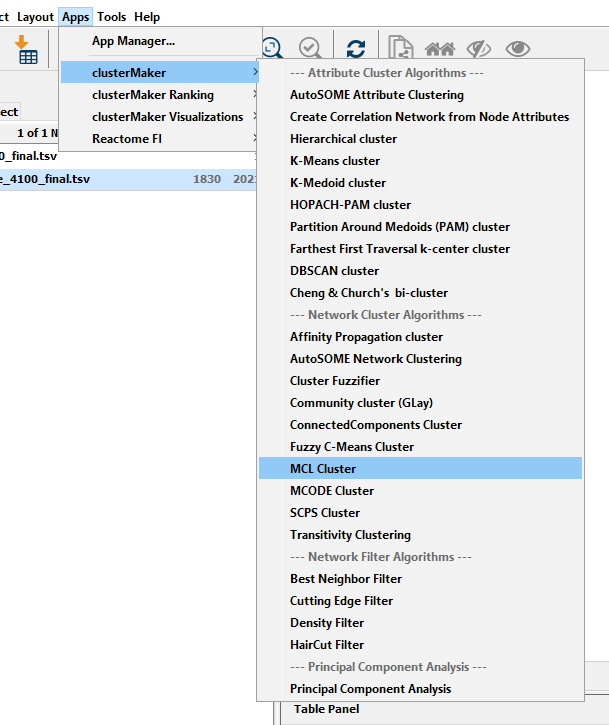
\includegraphics[width=15cm]{6-cluster}
\end{figure}

This is the view after clusterMaker2 has run the \textit{MCL cluster} method on
the current network. As seen on the left side menu, a new network has been
listed. This network only appears if the user sets the "Create new clustered
network"-option in the clustering parameter dialog that appears after choosing a
clustering algorithm from the clusterMaker2 menu.
\begin{figure}[H]
    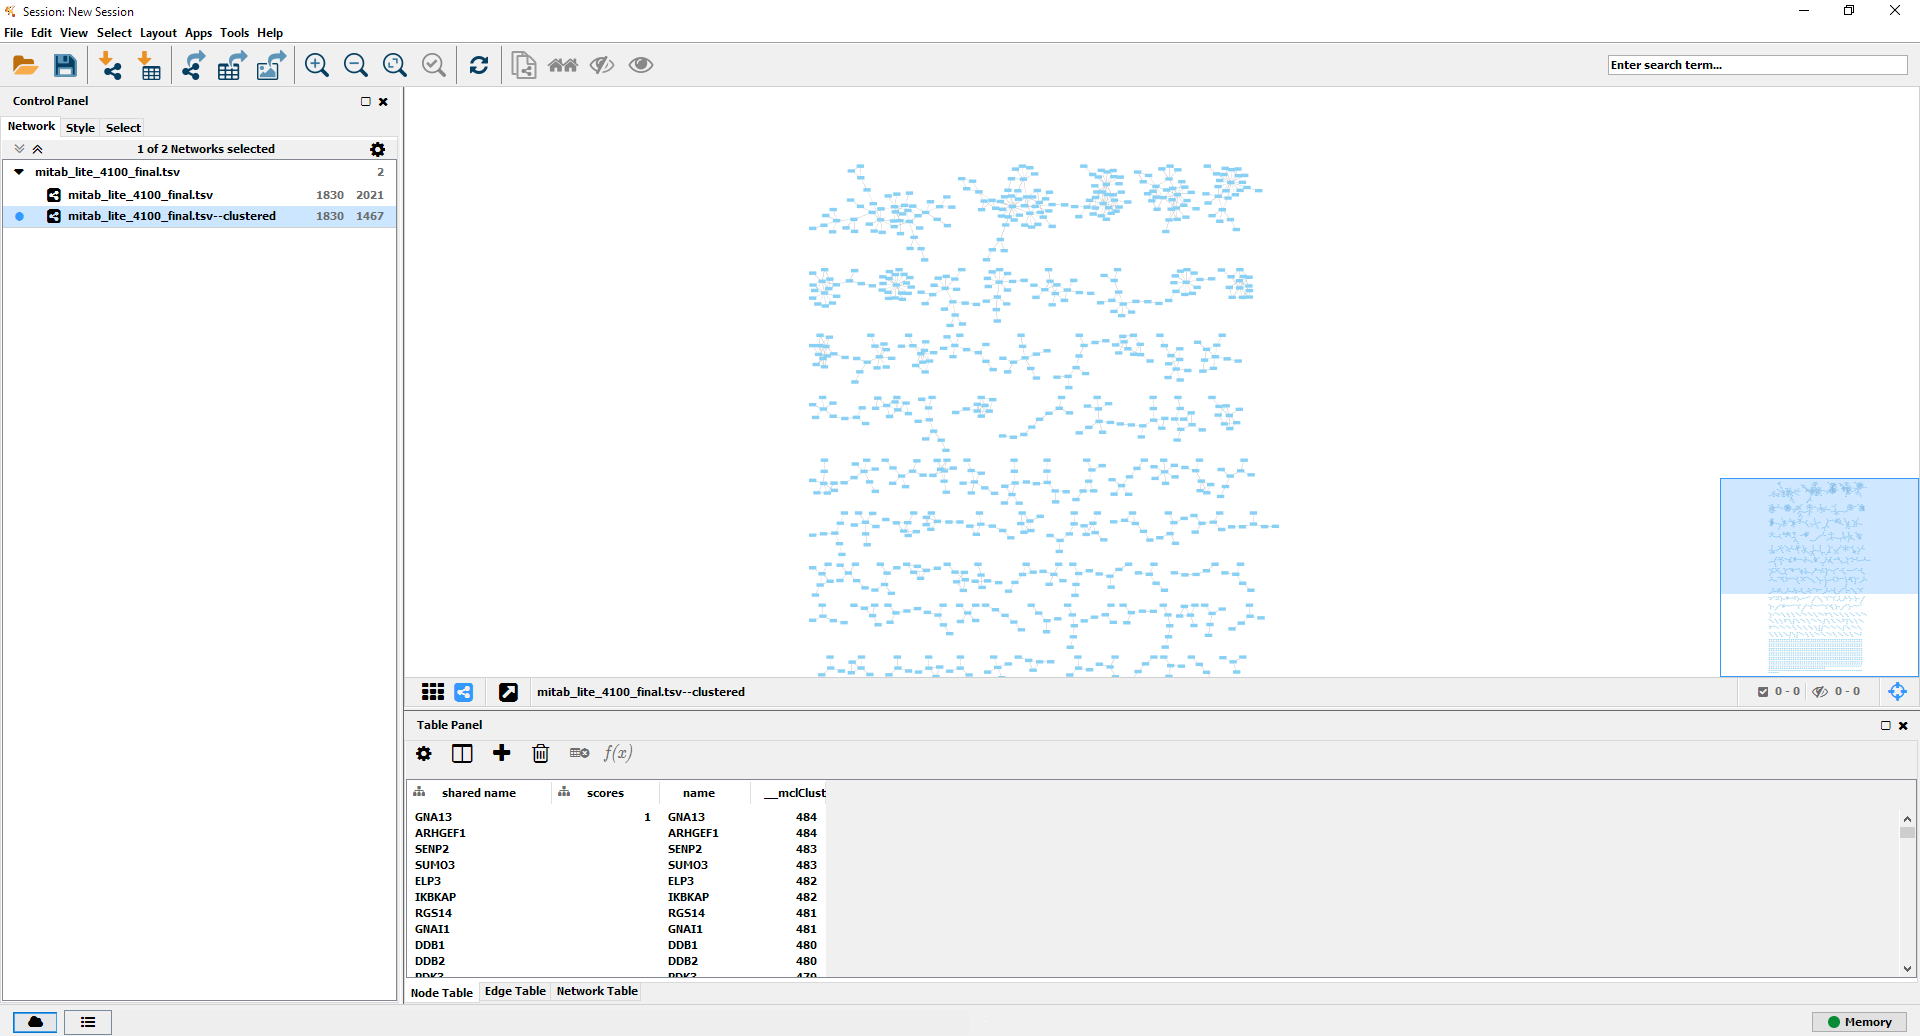
\includegraphics[width=15cm]{7-done-cluster}
    \label{fig:done-cluster}
\end{figure}

Here the cluster ranking algorithm menu is shown.
\begin{figure}[H]
    \label{fig:choose-ranking}
    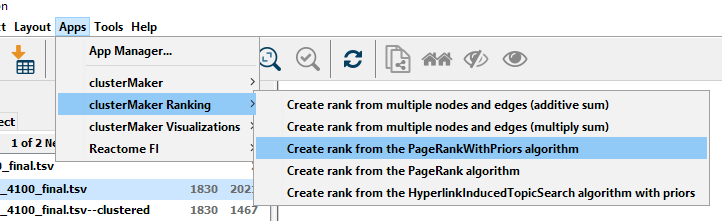
\includegraphics[width=15cm]{8-choose-ranking}
\end{figure}

The \gls{prwp} was chosen as the ranking algorithm. Node and edge attributes can
be combined by the user in any way.
\begin{figure}[H]
    \label{fig:pagerank}
    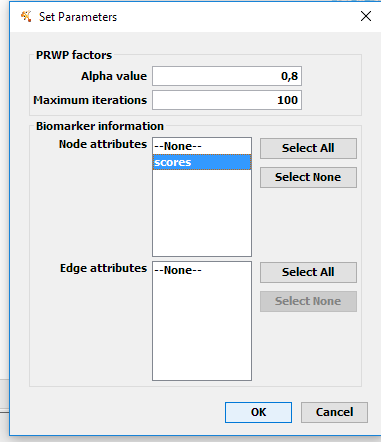
\includegraphics[width=15cm]{9-pagerank}
\end{figure}

If the user is interested in visualizing the ranks, it is possible to click the
"Show results from ranking clusters" option in the visualization menu. No menu
will appear after that, but rather will Cytoscape open a loading dialog similar
to when clustering and ranking algorithms has been tasked to start.
\begin{figure}[H]
    \label{fig:show-results}
    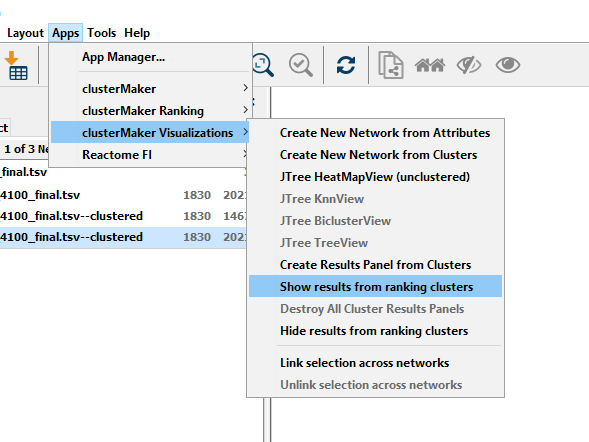
\includegraphics[width=15cm]{10-show-results}
\end{figure}

Here is the results panel displaying the ranked clusters from top to bottom,
descending scores. The title for each results panel is formatted as in the
example.
\begin{Verbatim}[fontsize=\scriptsize]
[<clustering algorithm>]{<ranking algorithm>}(<network name>)
\end{Verbatim}
So with MCL clustering, \gls{prwp} ranking and the
"mitab\_lite\_4100\_final.tsv--clustered" network, this is what the title
becomes:
\begin{Verbatim}[fontsize=\scriptsize]
[mcl]{PRWP}(mitab_lite_4100_final.tsv--clustered)
\end{Verbatim}
As seen in the title. The coloring has been discussed earlier.
\begin{figure}[H]
    \label{fig:result-colors}
    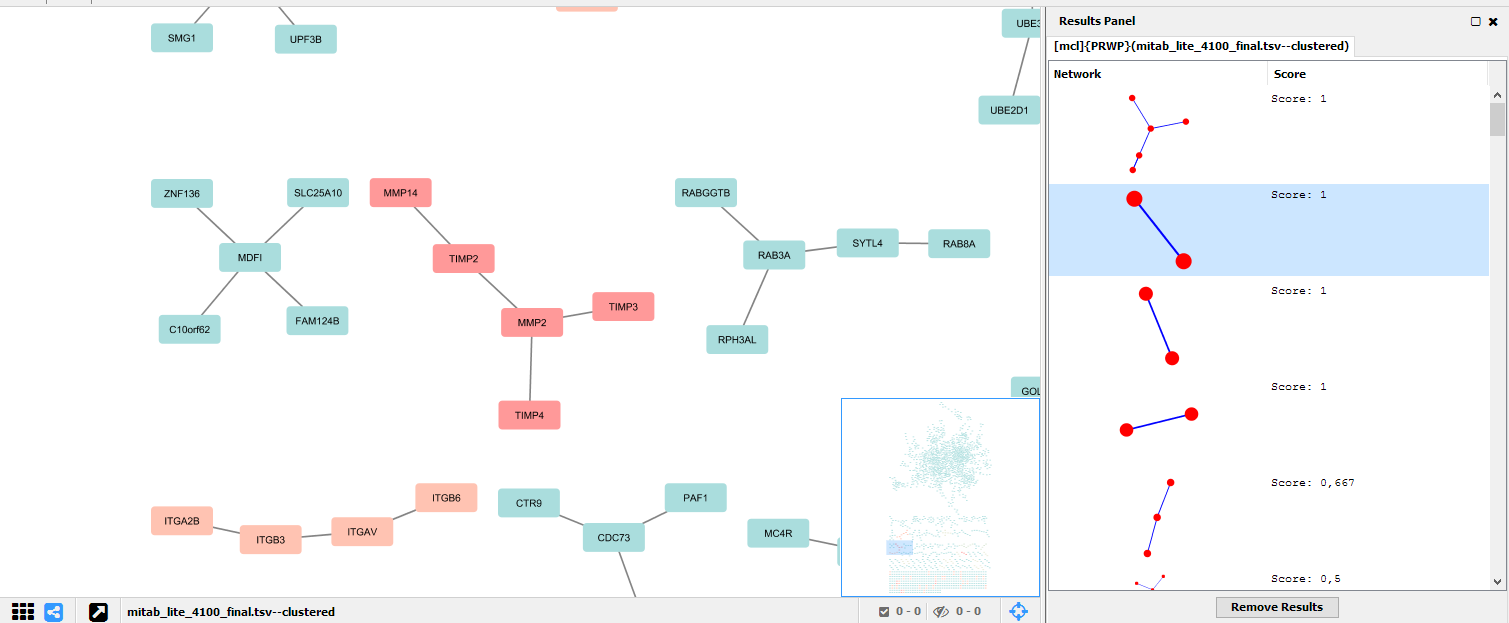
\includegraphics[width=15cm]{11-result-colors}
\end{figure}

Here is an example of how the clusters change color when selected from the
results panel menu.
\begin{figure}[H]
    \label{fig:rank-selection}
    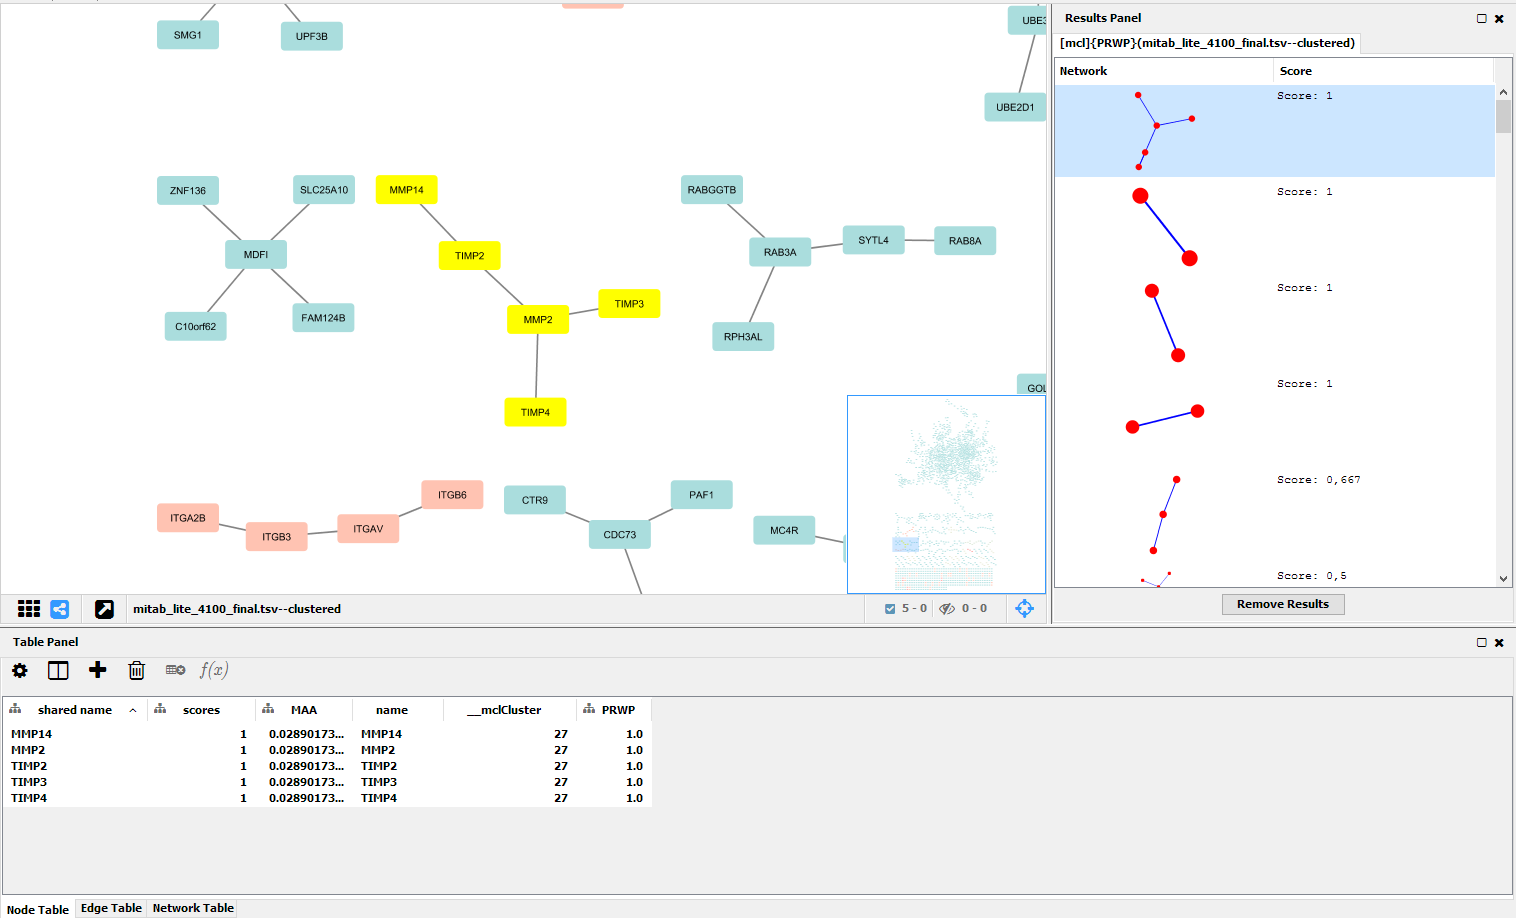
\includegraphics[width=15cm]{12-rank-selection}
\end{figure}

\section{Design}
\begin{figure}[H]
    \caption{Ranklust ranking algorithm relations}
    \label{fig:rank-alg}
    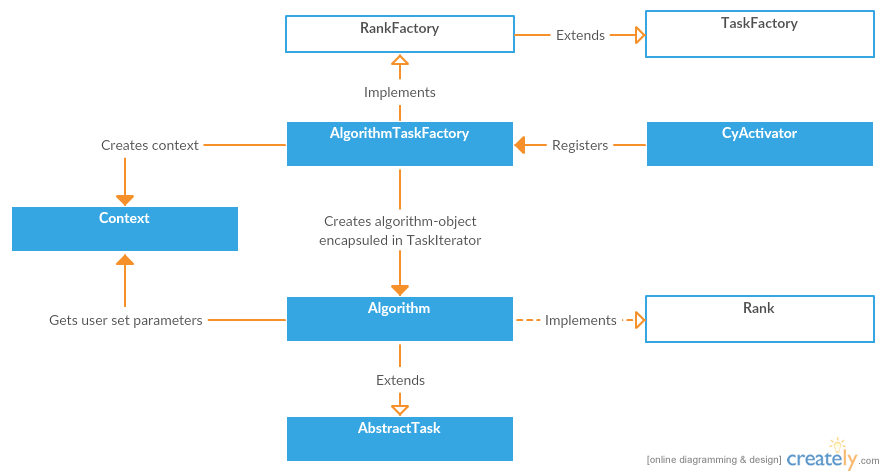
\includegraphics[width=\textwidth]{ranklust-algorithm}
\end{figure}
\begin{figure}[H]
    \caption{Ranklust ranking panel relations}
    \label{fig:rank-panel}
    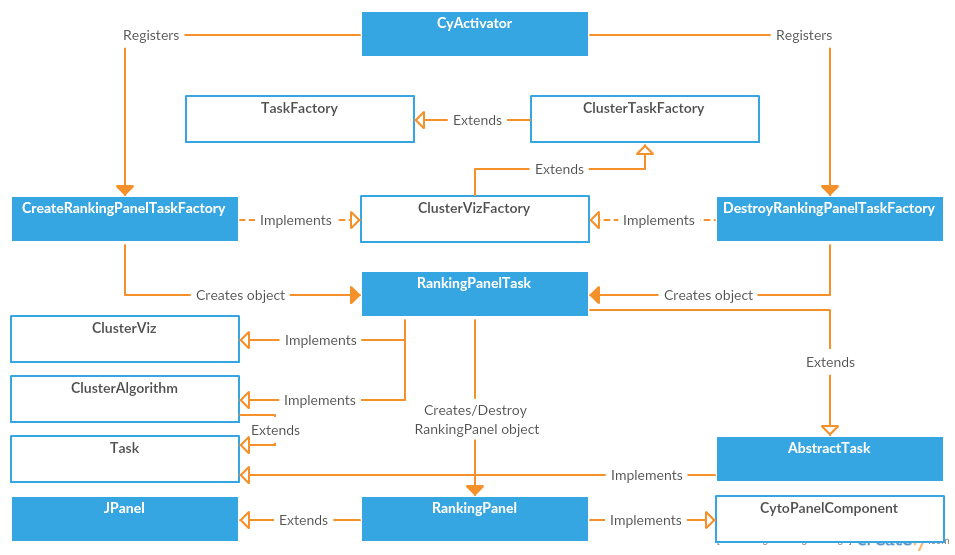
\includegraphics[width=\textwidth]{ranklust-panel}
\end{figure}

\chapter{Identifying network biomarkers through graph analysis}
\section{How the network was created}
After querying iRefWeb for the PPI-network with the query displayed earlier
(figure \ref{fig:irefweb}) the resulting network consisted of 109276 interactions.
After filtering the same network through the protein-to-gene mapping constructed
from HGNC, the final network consisted of 9500 nodes (genes) and 43706 edges
(interactions). At this point, all of the nodes and edges were undirected and
unweighted. Converting from proteins to genes ended up with a 60\% perturbation
of the network in the form of removed edges. Clustering the network resulted in
a further perturbation of 69.8\% of edge-removal when compared to the
HGNC-filtered network, 87.9\% when compared to the unfiltered iRefWeb network.

The creation of the \gls{golden} through combining DisGeNET and \gls{dragon}
resulted in a file with two columns. One representing a gene, the second one
representing the score of a gene, so a single row would contain a unique gene in
the list and the score it received.

\section{Which parameters for clustering was used and why}
Talking about \gls{mcl} results
\begin{table}[H]
    \centering
    \begin{tabular}{| l | p{2cm} | p{2cm} | p{2cm} | p{2cm} | p{2cm} | p{2.1cm} |}
        \hline
        \textbf{Inflation} & \textbf{Clusters} & \textbf{Avg.  cluster size} &
        \textbf{Max. cluster size} & \textbf{Min. cluster size} &
        \textbf{Modularity} \\
        \hline
        1.6 & 1068 & 8.88 & 968 & 2 & 0.367 \\
        1.8 & 1400 & 6.60 & 660 & 2 & 0.307 \\
        2.0 & 1599 & 5.68 & 405 & 2 & 0.269 \\
        2.5 & 2053 & 4.20 & 179 & 2 & 0.223 \\
        3.0 & 2210 & 3.75 & 122 & 2 & 0.199 \\
        \hline
    \end{tabular}
    \caption{MCL clustering parameter and statistic results}
    \label{tab:mcl-inflation}
\end{table}
The modularity of the clustered networks gives an indicator of how well the
process of creating the clusters went. Modularity is given as a score from 0 to
1. A score closer to 1 is more preferrable, as this indicates that the clusters
created have a good degree of separation to the other clusters in the network.
The preferred score to end up with would be around 0.8, but in this network
there has been a good amount of perturbation through the protein-to-gene
process. Modularity is not the only indicator of how well a network was
clustered, hence the choice of not setting the inflation value in \gls{mcl} to
1.6, but rather 1.8. When a lower inflation value is set, \gls{mcl} does not
separate edges between nodes as vigorously and as a direct cause, inflation will
go up. Taking the other attributes in the table (table: \ref{tab:mcl-inflation}) into
consideration, 1.8 seemed like the best inflation value. An inflation value of
1.8 has also been proved to be good for large high-throughput constructed
protein-protein networks with a large amount of alterations\cite{mcl-inflation}.

The amount of iterations used for \gls{mcl} ended up being 200. It started out
at 1000, but the results converged somewhere between 170 and 200 iterations, so
it was decreased form 1000 to 200 to speed up the time used in the
\gls{pipeline}.

\section{Results from cross-validation and what they indicate}
\begin{sidewaysfigure}
    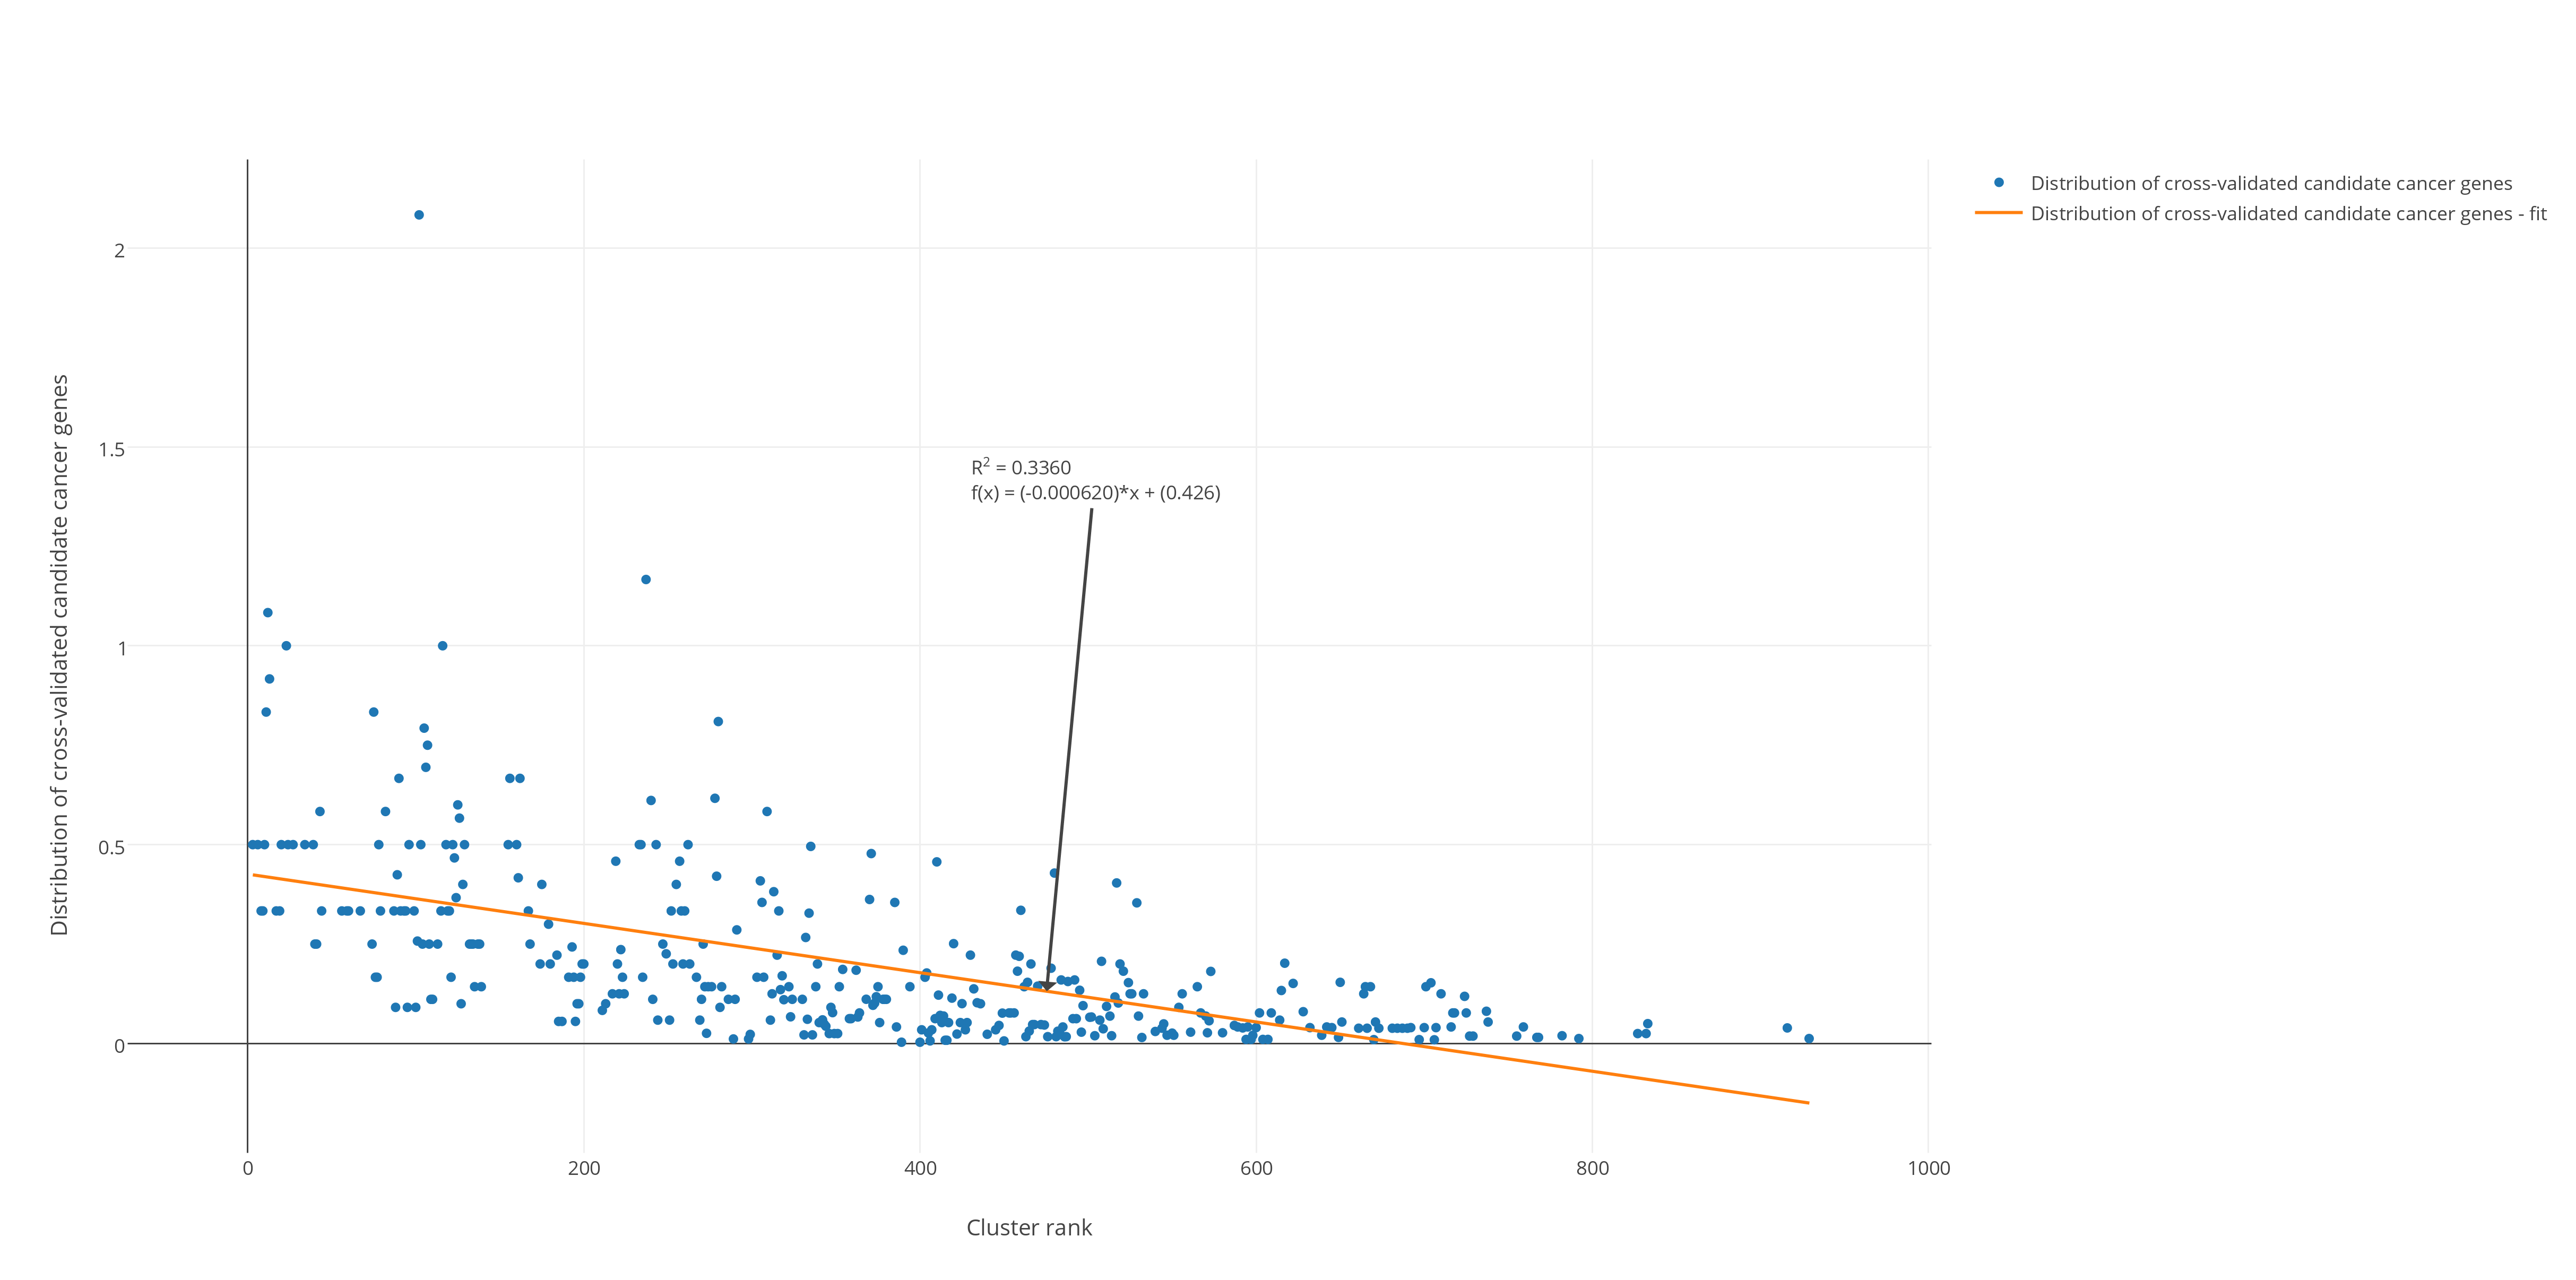
\includegraphics[scale=0.63]{cv_dist_total_filtered_prwp}
    \label{fig:irefweb-prwp}
    \caption{Distribution of combined averages of genes, which had their scores
    removed by cross-validation, ranked by PRWP}
\end{sidewaysfigure}

\begin{sidewaysfigure}
    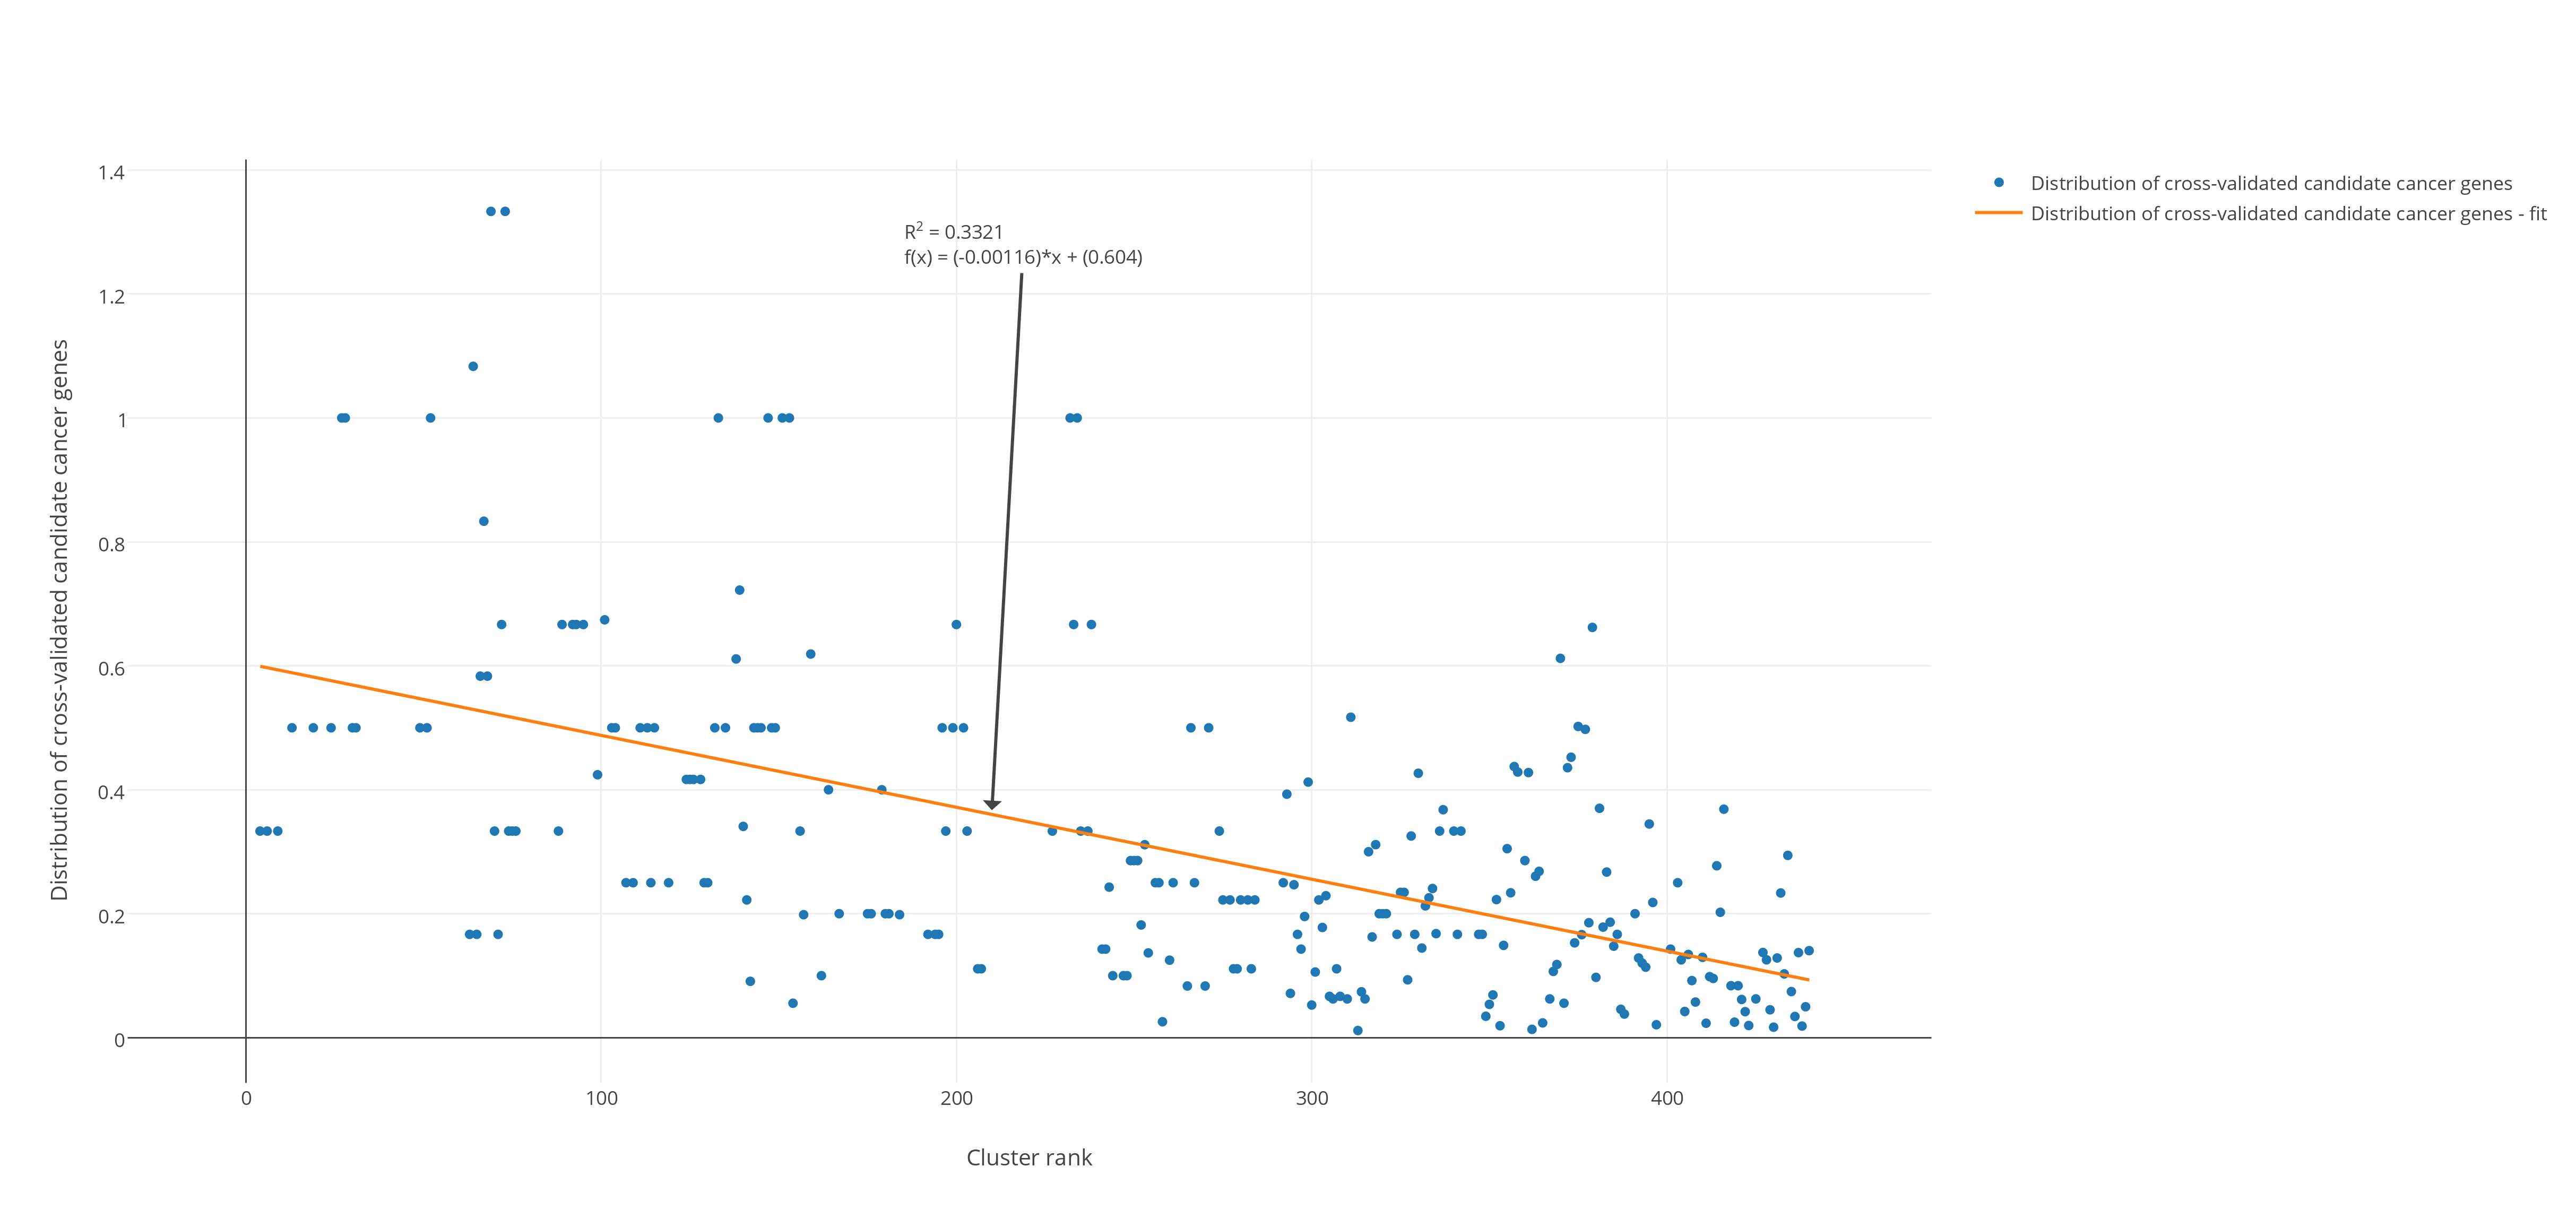
\includegraphics[scale=0.63]{cv_dist_total_filtered_maa}
    \label{fig:irefweb-maa}
    \caption{Distribution of combined averages of genes, which had their scores
    removed by cross-validation, ranked by MAA}
\end{sidewaysfigure}

The plots in figure \ref{fig:irefweb-prwp} and figure \ref{fig:irefweb-maa} is
developed from the 10 random cross-validation runs ranked with \gls{prwp} and
\gls{maa}. The x-axis represents the cluster ranks which is represented as
a blue dot in the scatter plot. Each rank consists of a single cluster which has
an arbitrary number of genes above 1. The y-axis represents a result from two
steps. The first step was to go through each of the
10 cross-validated results from ranking the iRefWeb network with \gls{prwp} and
\gls{maa}. In each of the cross-validated results an average was calculated for
each cluster. The average was calculated from dividing the number of genes, that
had their prior score removed as a result of the cross-validation, by the total
number of genes in the cluster. Each cluster would at this point have an average
representing the average of cross-validated genes in a cluster. The second step
completes the values for the y-axis in the plot and represents the score in
a cluster when additively combining the averages from each of the 10
cross-validated results that was found by \gls{prwp} and \gls{maa}. To filter
out the uninteresting results, all zero values on the y-axis was removed.

The analysis of which clusters contained the largest combined average of genes,
which had their prior score removed by cross-validation, shows that the topmost
ranked clusters had the highest combined average. This information indicates
that ranking clusters with \gls{prwp} and \gls{maa} have a tendency towards
ranking the larger part of the population of prostate cancer biomarkers at the
top of the cluster ranks, and the lower at the bottom.

Executing a cross-validation on the iRefWeb with \gls{prwp} and \gls{maa}
rankings had two purposes. The first being to prove the fact that every gene
that had its prior score removed by the cross-validation, should be found in the
results of the cluster ranking and identified as candidate biomarkers. The
second, to prove that the distribution of the combined average in the clusters
should correlate to the rank they obtained through Ranklust's use of \gls{prwp}
and \gls{maa}.

\subsection{Differences between ranking with PRWP and MAA}
There is clearly a trend in both \gls{prwp} and \gls{maa}. The difference
between them being mainly the number of clusters ranked and the coupling of
values around the linear regression fit. It is important to point out that this
is just a result over the distribution of candidate cancer genes at certain
ranks. Where the clusters resides in the rankings may be very different between
the \gls{prwp} and \gls{maa}.

The values in \gls{prwp} have a tighter coupling, in other words, the distance
the coordinates have in the scatter plot deviate less from the fit than the ones
in the \gls{maa} plot. The difference is not huge, as the coefficient of
determination indicates 0.336 in \gls{prwp} against 0.332 in \gls{maa}. Both
ranking algorithms achieves a descending distribution of cross-validated genes
from the topmost to the lowest ranked cluster. Though, when comparing the
cross-validation results between \gls{prwp} and \gls{maa}, \gls{prwp} comes out
ahead by a margin in \gls{rsquared} value.

\section{Benchmarking Ranklust against text mined, curated knowledge and experimental test data}
\subsection{Retrieving the test data from the DISEASE database}
Benchmarking Ranklust is done against three resources of data from a single
database called DISEASE\cite{jensen}. This database can be queried for diseases
or genes. The query in this database was limited to searching for a single
disease or gene name. No API was found to access the database directly, so to
retrieve the gene names related to prostate cancer, whole files was downloaded.
There were three files, one for each type of research put into retrieving the
data: text mined, manually curated knowledge and experimental data. Each of
these files was filled with genes and their relation to different diseases, so
they had to be filtered to only contain genes with information about prostate
cancer. This was done by only using genes that contained "prostate cancer" in
the column indicating which disease the specific gene was related to.

The plots representing values in clusters from each of these three files have
split each cluster in two parts, blue and orange. The blue dots in the scatter
plot represents the genes in a cluster that has prior scores. The orange dots in
the scatter plot represent genes in the same cluster as the blue ones in terms
of which rank they are in based on the x-axis, but they do not have prior
scores. The blue dots are also mentioned as prostate cancer genes and orange
dots as prostate candidate cancer genes, because they have no score, but they
are in some cases related to other prostate cancer genes to such a degree that
they are susceptible to be candidate cancer biomarkers for prostate cancer. As
with the cross-validation plots, the zero values in the plots have been removed.

\subsection{Z-scores for text mined genes in clusters}
\begin{sidewaysfigure}
    \label{fig:txt-iref-prwp}
    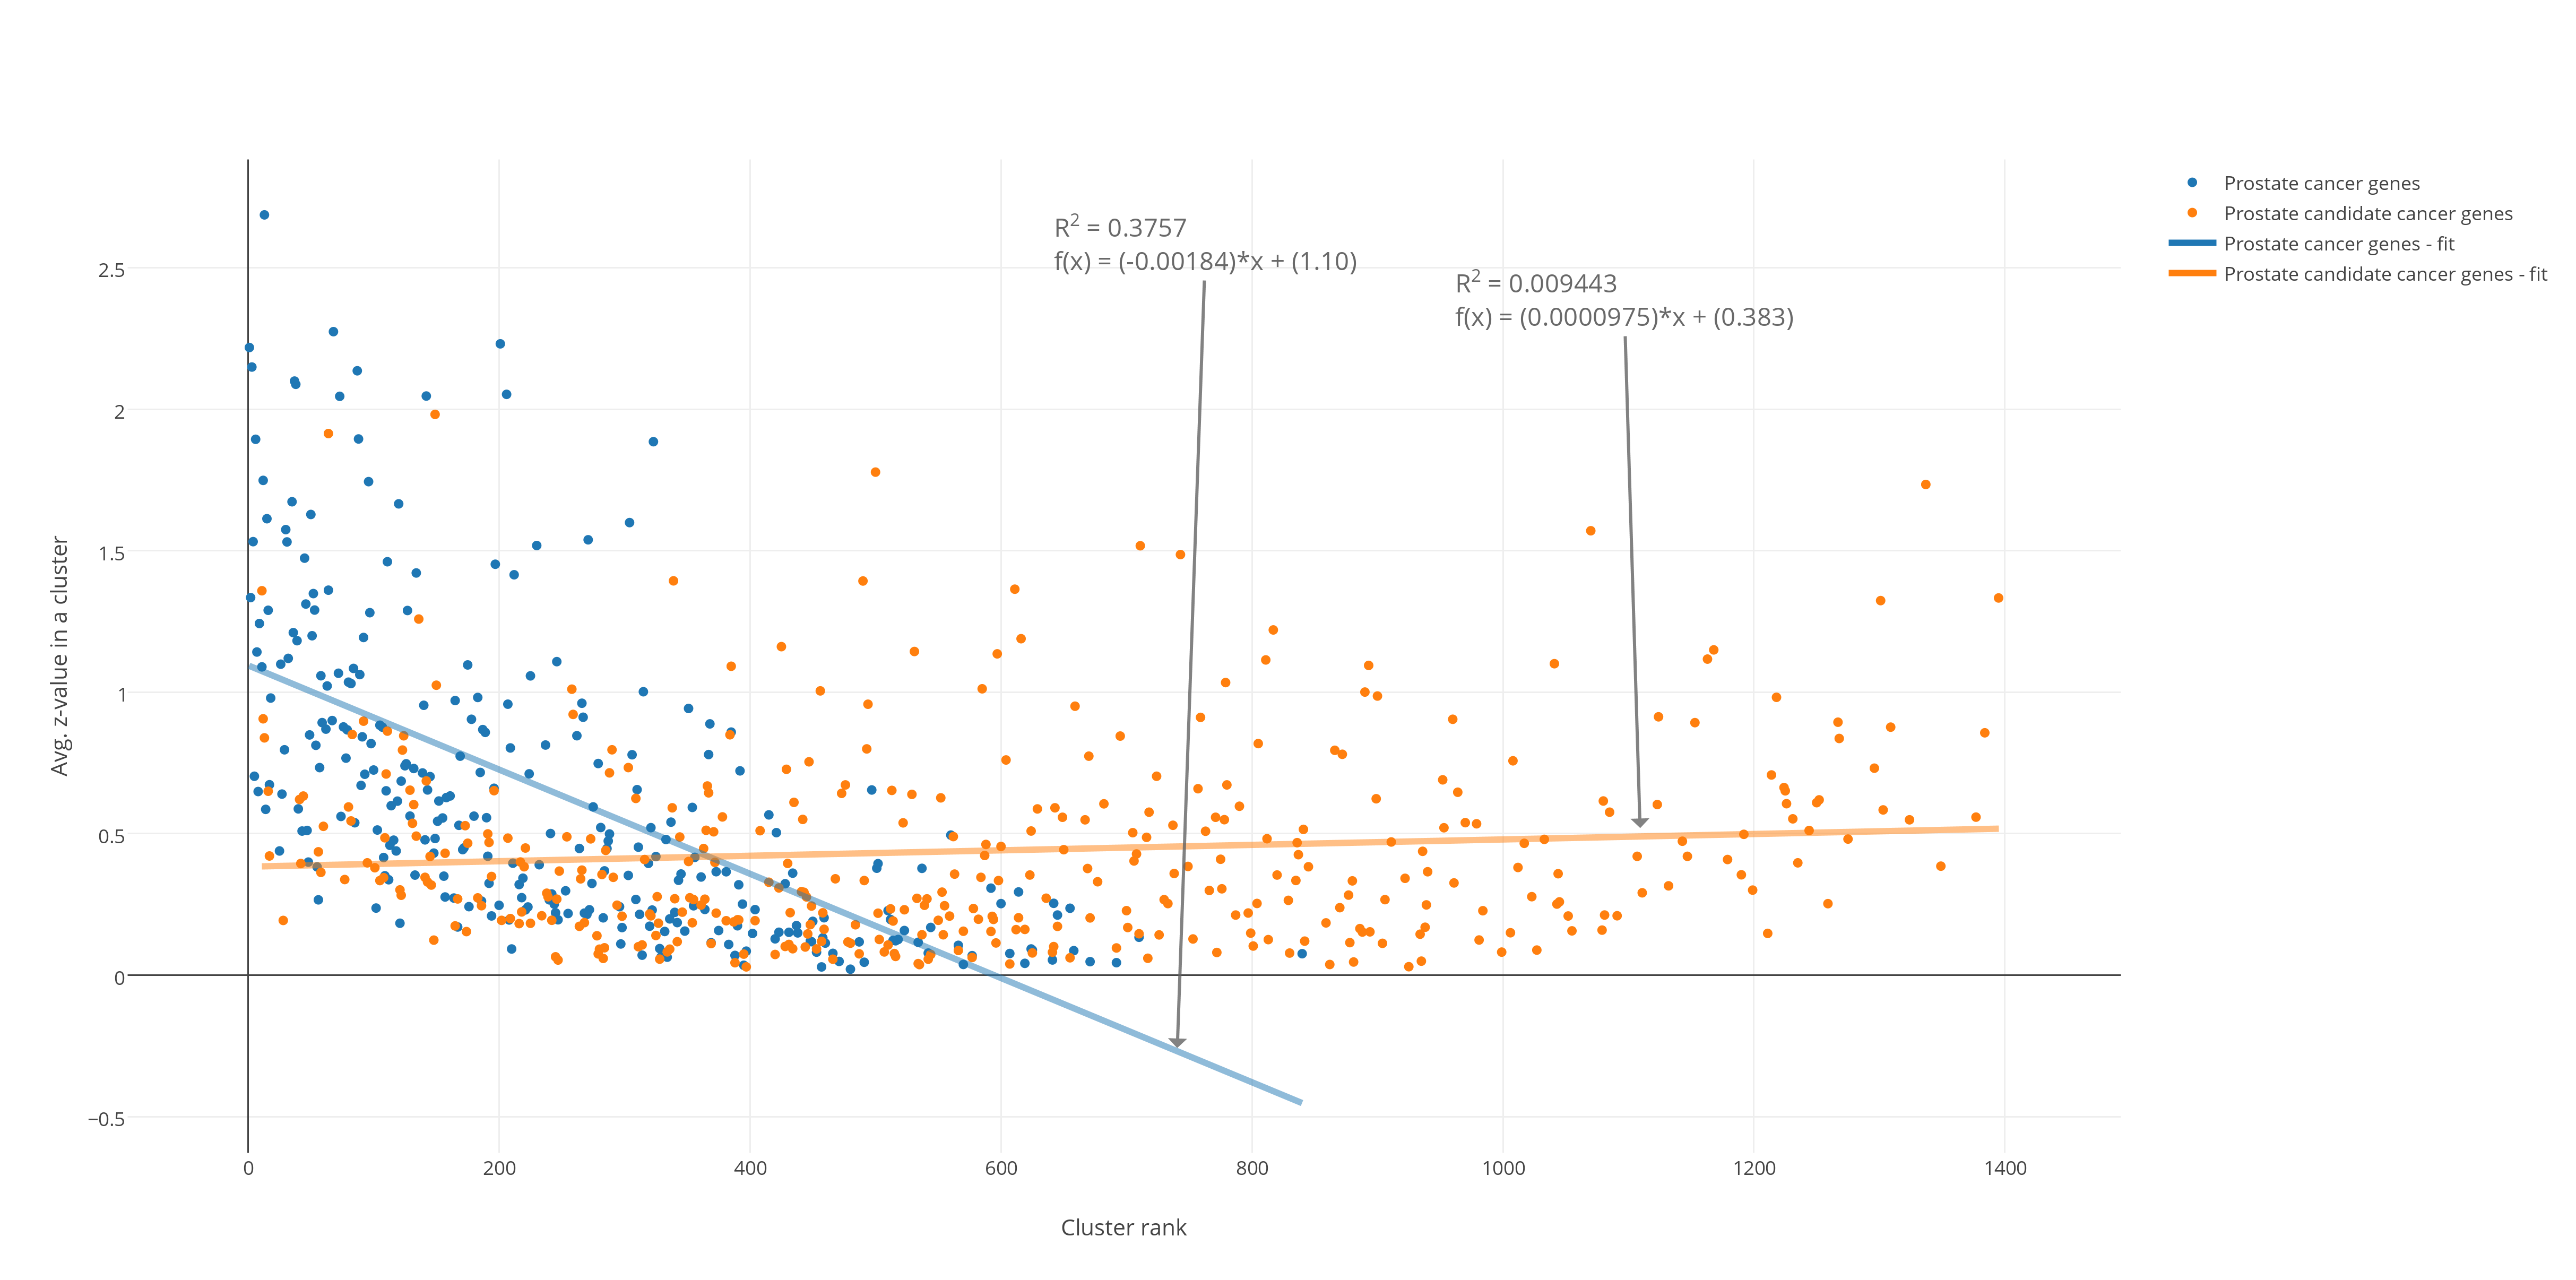
\includegraphics[scale=0.63]{prwp_txt_split}
    \caption{Average z-score in a cluster ranked by PRWP}
\end{sidewaysfigure}
\begin{sidewaysfigure}
    \label{fig:txt-iref-maa}
    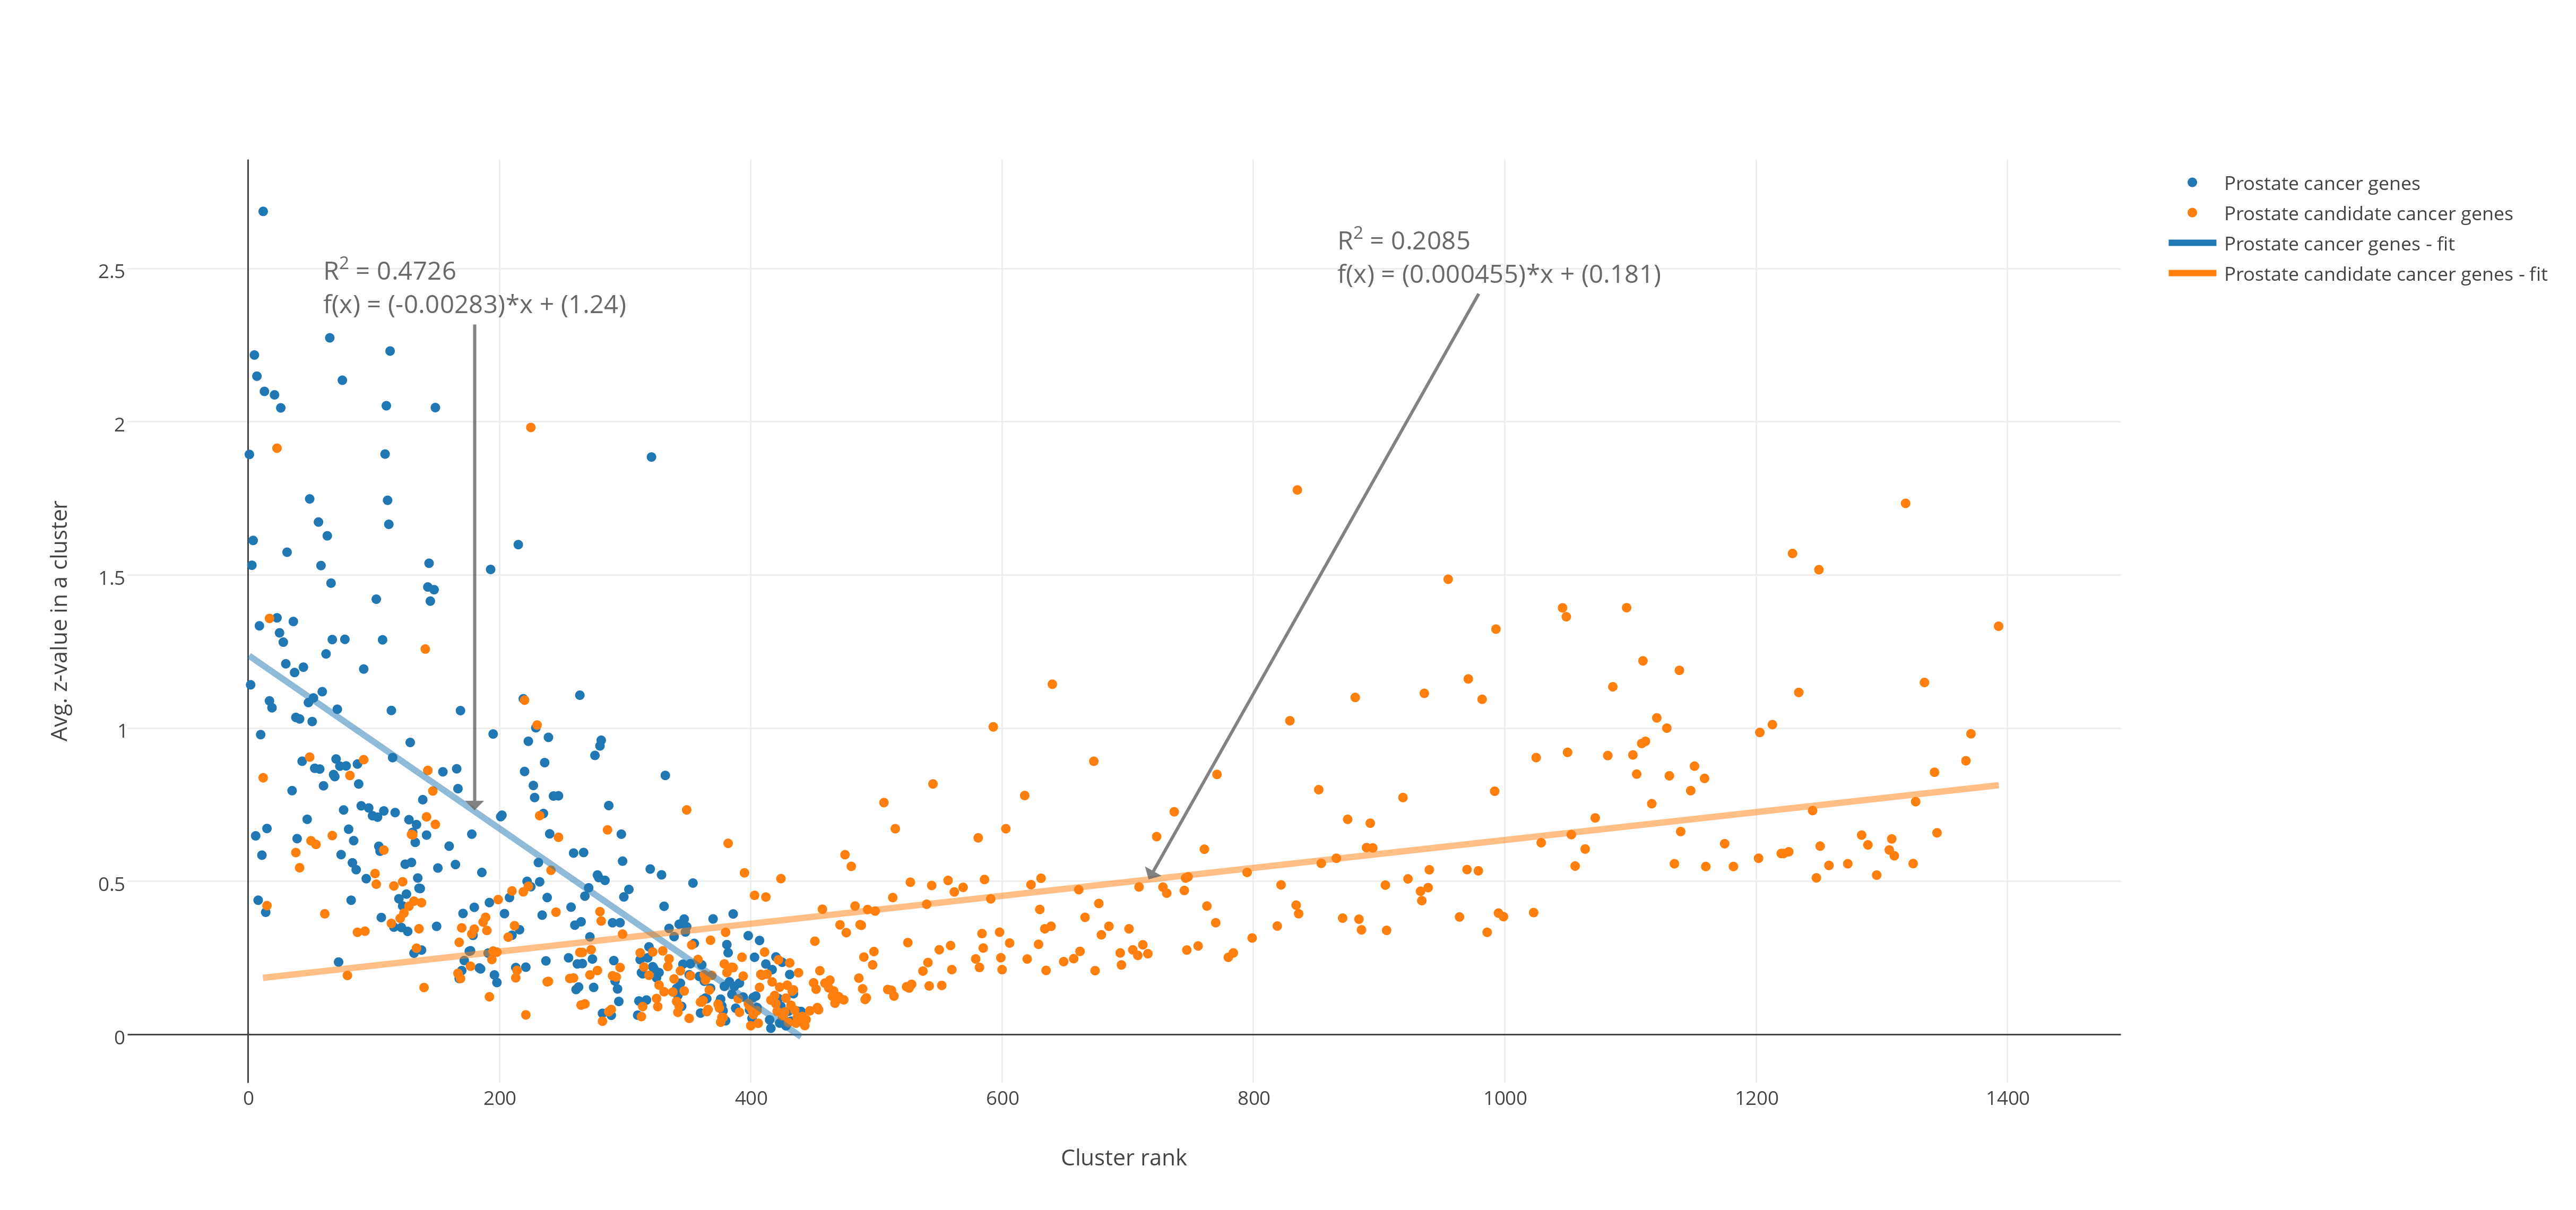
\includegraphics[scale=0.63]{maa_txt_split}
    \caption{Average z-score in a cluster ranked by MAA}
\end{sidewaysfigure}

The text mined scores are represented by a z-score. The z-score to a gene in the
text mined data from the DISEASE database is a developed from a co-occurence
score, which increased when a gene and a disease was mentioned together, but
also decreased when they were mentioned with multiple other genes or diseases.
This co-occurence score was later converted to z-scores to be more robust to
changes to the size of the text corpus in the DISEASE database\cite{jensen}.
This results in the average z-score to a cluster, which is based on the average
z-score of each gene in a cluster, to be a benchmark as to how high the cluster
should be ranked in terms of being a relevant network biomarker for prostate
cancer.

Since the plots have split each cluster into two parts, the cluster part of
genes with priors and the ones without priors, the expected outcome, should the
ranking algorithms perform as expected, would be to have the blue dots
descending and the orange dots ascending, when looking at a linear regression
fit going from the topmost ranked cluster to the lowest.

\subsubsection{PRWP benchmarked with text mined genes}
For \gls{prwp} (figure: \ref{fig:txt-iref-prwp}), the prostate cancer candidate genes is
descending in z-values from the topmost ranked cluster to the lowest, which is
contributing to showing \gls{prwp}'s suitability for ranking clusters as
candidate biomarkers.

The prostate candidate cancer biomarkers are ascending in z-value from the
topmost to the lowest ranked cluster. High z-values could contribute to the fact
that ranklust has found actual prostate candidate cancer biomarkers. However,
a low z-values does not contradict it. The only fact to deduce from low z-values
is that they have not been examinated to the degree that they are not mentioned
as a single gene related to prostate cancer in scientific papers.

\subsubsection{MAA benchmarked with text mined genes}
For \gls{maa} (figure: \ref{fig:txt-iref-maa}), the prostate cancer genes have the same
distinct descension in z-values from the topmost to the lowest cluster ranks.
The difference from \gls{prwp} to \gls{maa} being that \gls{maa} has a more
distinct ascending linear regresstion fit for the z-values in the prostate
candidate cancer genes.

\subsubsection{Conclusion of benchmarking through text mined genes}
This demonstrates the main difference between \gls{prwp} and \gls{maa}.
\gls{prwp} takes network structure into comparison as well as the prior scores,
so it will rank genes without priors higher than \gls{maa}. \gls{maa} focuses
purely on the prior scores, and so the network structure of protein complexes
are being completely ignored.

\subsection{Manually knowledge curated genes in a cluster}
\begin{sidewaysfigure}
    \label{fig:know-iref-prwp}
    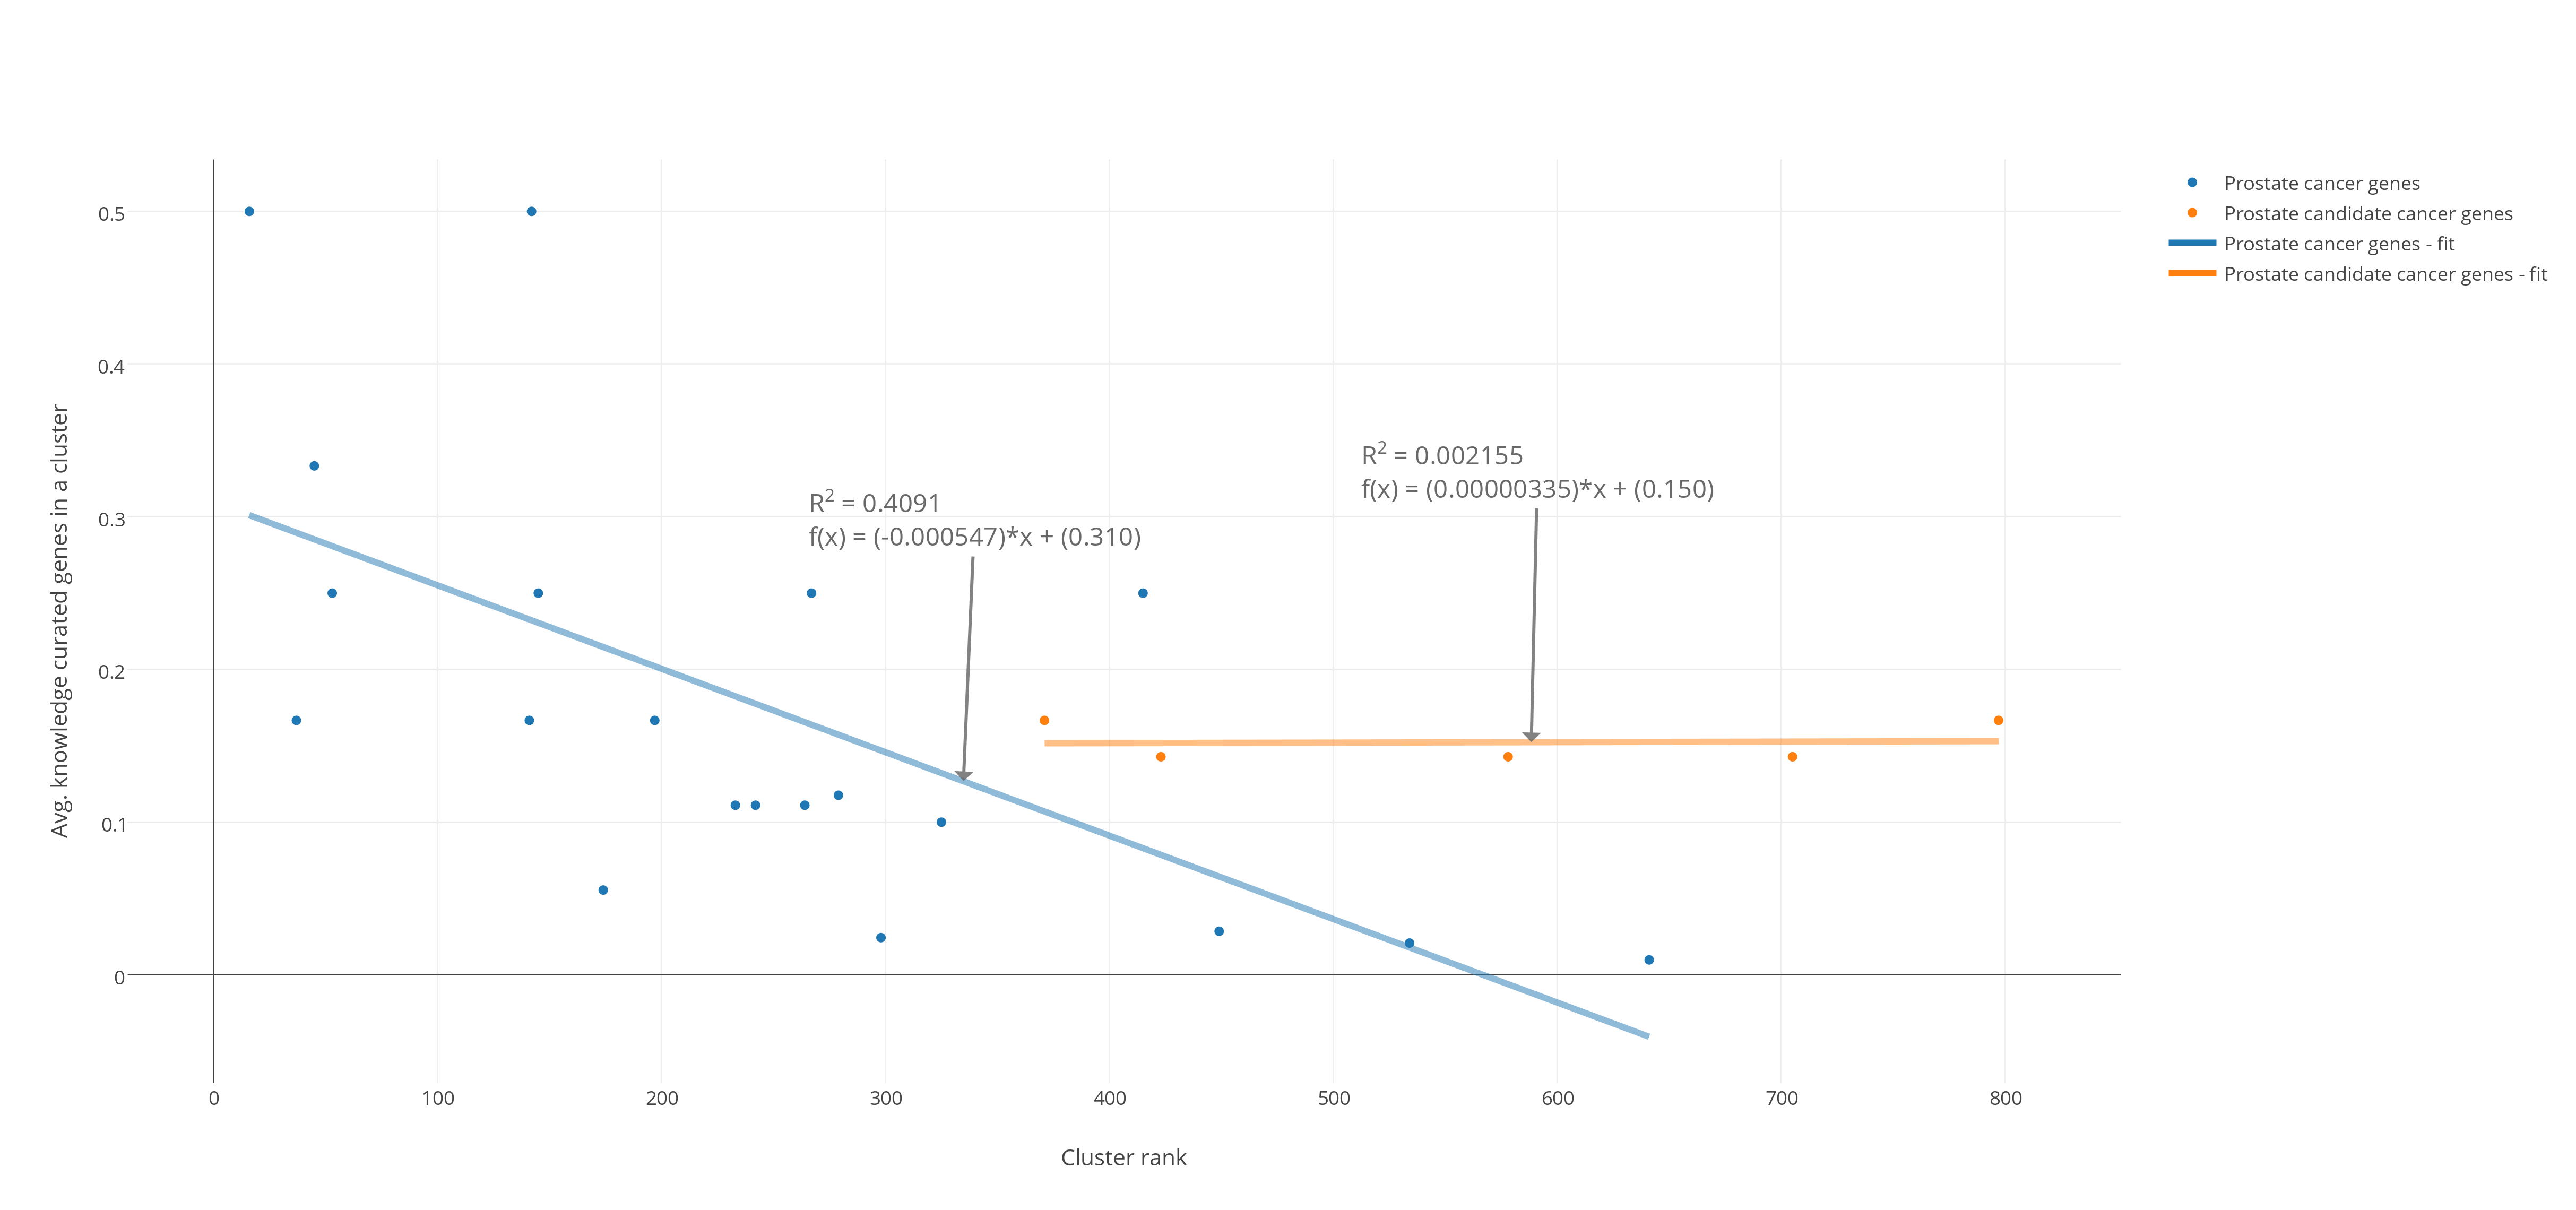
\includegraphics[scale=0.63]{prwp_know_split}
    \caption{Average distribution of curated knowledge mined genes in clusters
    ranked by PRWP.}
\end{sidewaysfigure}

\begin{sidewaysfigure}
    \label{fig:know-iref-maa}
    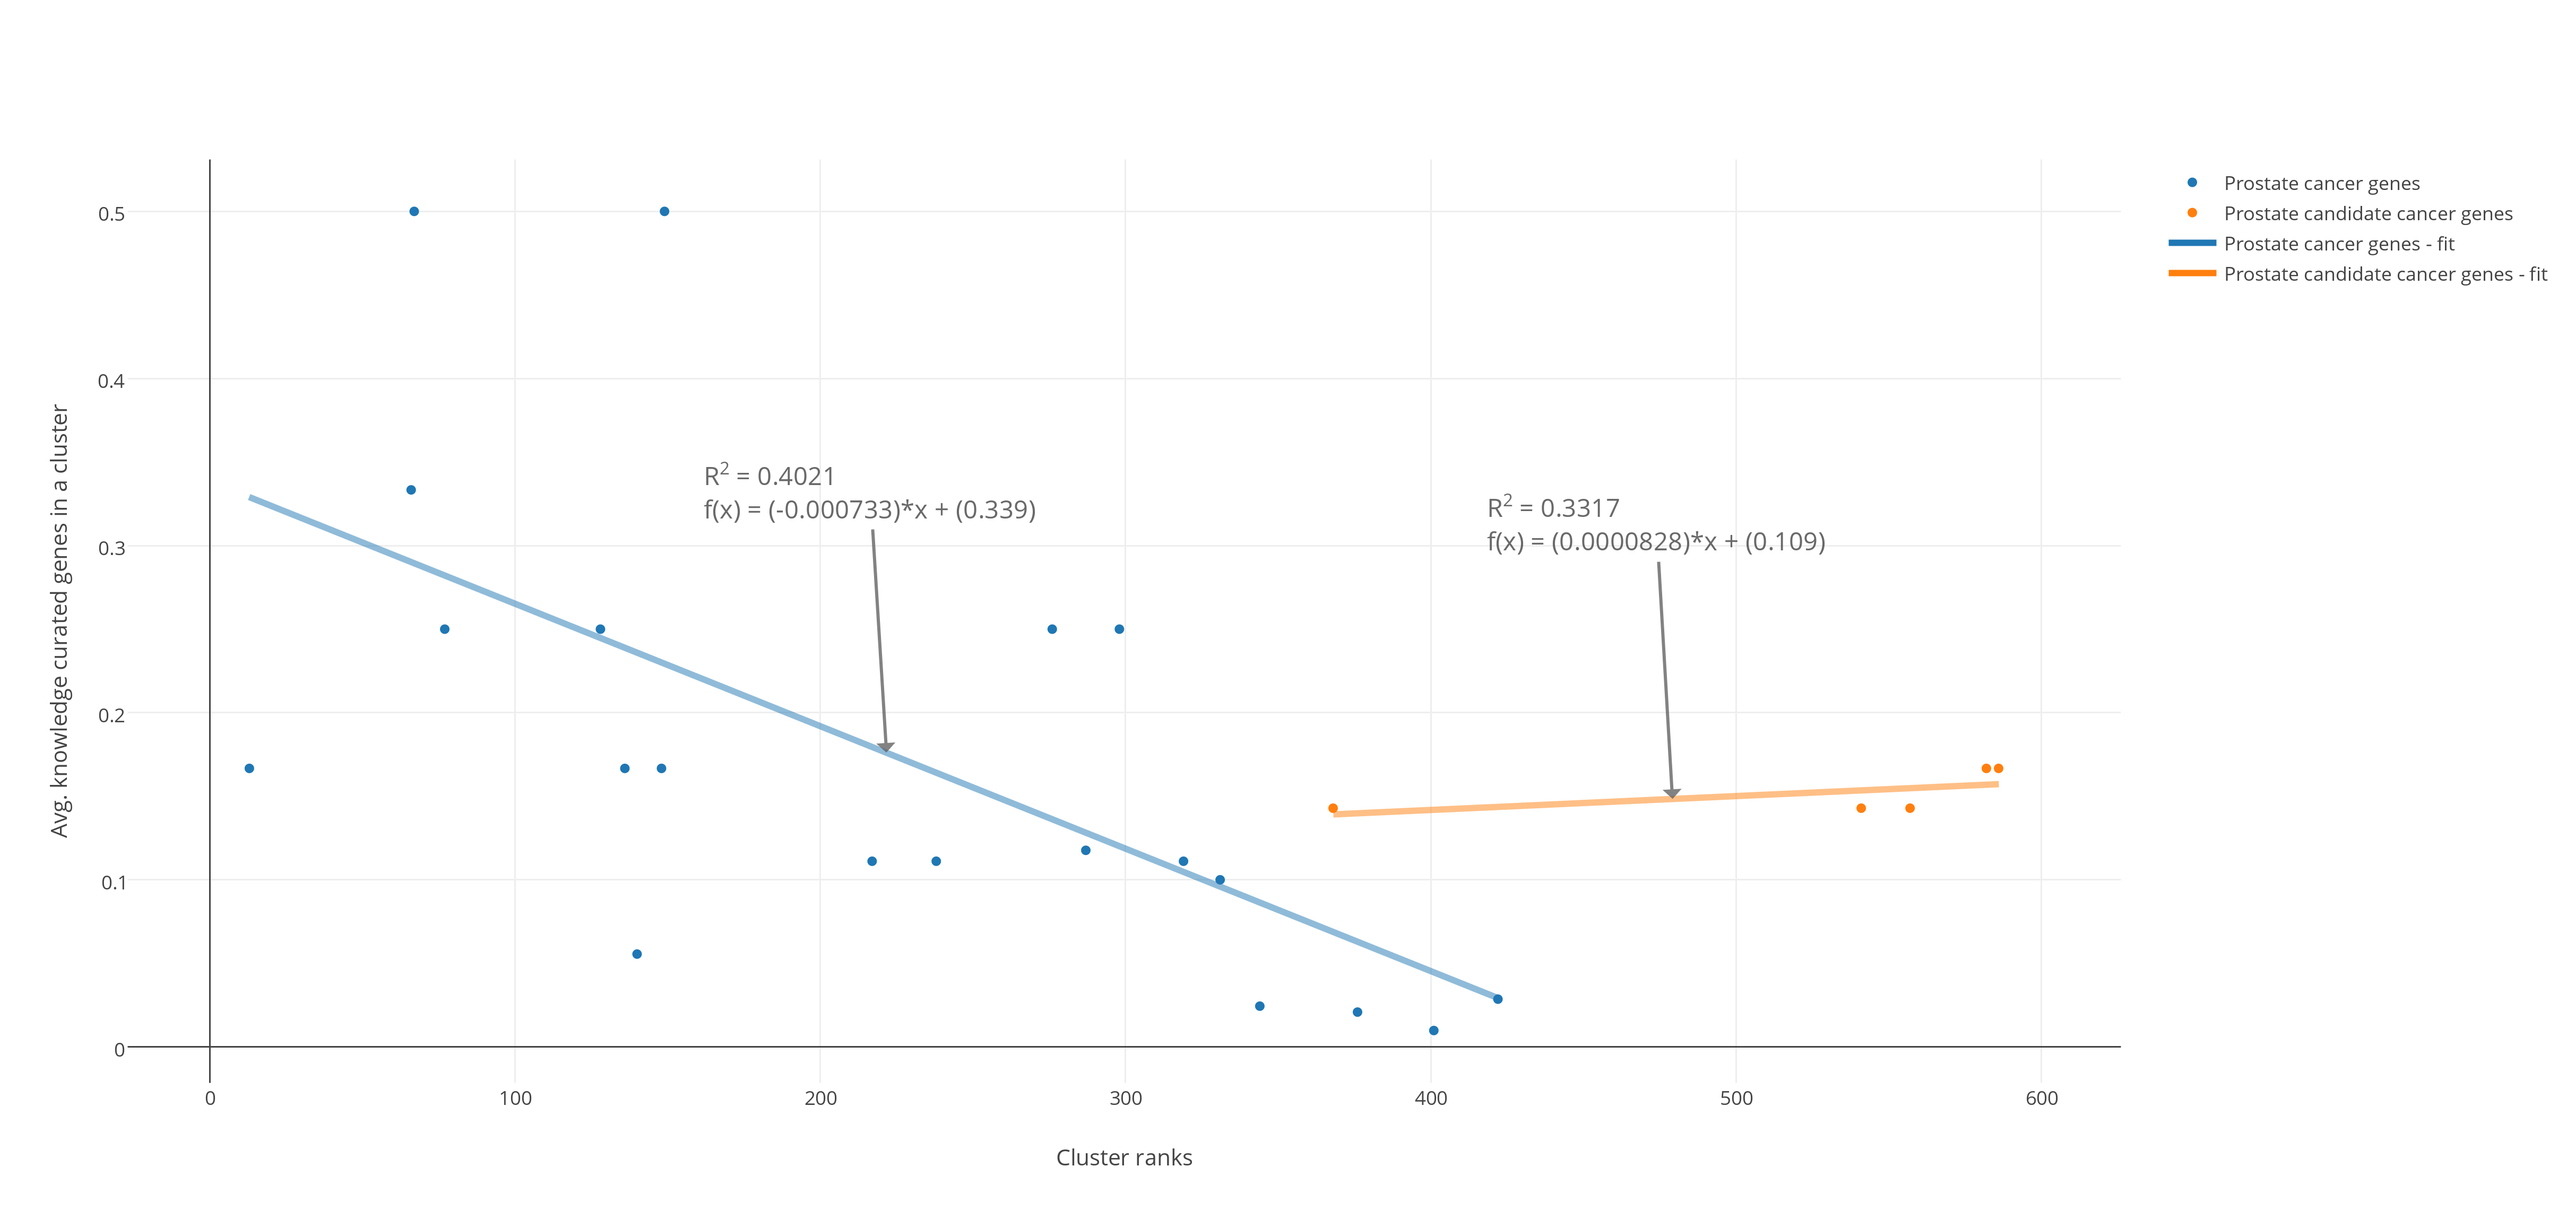
\includegraphics[scale=0.63]{maa_know_split}
    \caption{Average distribution of curated knowledge mined genes in clusters
    ranked by MAA.}
\end{sidewaysfigure}

This data had no score except for a confidence score in the \gls{jensen}
database. Every gene in the manually knowledge curated file had a confidence
score of 5 stars, due to being manually curated by researchers\cite{jensen}.
Therefore, the average number of genes in a cluster would receive a knowledge
score based on if the gene occurs in the knowledge curated part of the
\gls{jensen} database or not. So the knowledge curated data is only based on
occurence, and not a specific value, in contrast to the text mined and
experimentally mined genes in the database. The clusters are split two-ways, in
a similar way that the benchmark with the text mined genes was, blue for genes
in the cluster which have priors and orange for the genes that do not have prior
scores.

Another trait the knowledge curated data posssesses is the amount entries in the
\gls{jensen} database that has. Text mined data can be seen as the
high-throughput technology of retrieving relevant data from papers, while the
knowledge curated data is manually curated knowledge by researchers. This is why
the amount of entries for knowledge curated data is so sparse when compared to
text mined data.

For the manually knowledge curated genes to indicate valuable rankings of the
clusters, the genes with prior scores should have a descending trend from the
topmost ranked cluster to the lowest. If the genes without prior scores, have
a clear ascending trend from the topmost to the lowest ranked cluster, it would
have been a direct contradiction to the fact that the ranking algorithms should
be able to rank genes without prior scores in a reasonable way if they are
related to genes with priors. A higher frequency of manually knowledge curated
genes would increase the validity of these thrends, should they occur,
especially if they are subtle.

\subsubsection{PRWP benchmarked by manually knowledge curated genes}
For \gls{prwp} (figure: \ref{fig:know-iref-prwp}), the genes with prior scores in
a cluster have a clear descending trend from the topmost to the lowest ranked
cluster. This builds up under the validitiy of \gls{prwp} being able to rank
prior scored genes correctly. The genes without prior scores in a cluster does
ascend to a low degree and the \gls{rsquared} for the fit that has this
ascending trend is not deemed as a good fit for the scores, at a \gls{rsquared}
value of only 0.002.

\subsubsection{MAA benchmarked by manually knowledge curated genes}
For \gls{maa} (figure: \ref{fig:know-iref-maa}), the genes with prior scores in a
cluster have the same trend as in \gls{prwp}. For the genes without prior scores
in a cluster, the trend also is the same as in \gls{prwp}, but to a higher
degree. The fit for the ascending average in manually knowledge curated genes in
a cluster, for the genes in the cluster without prior scores is an
\gls{rsquared} value of 0.33, which is considerably higher than the ascending
value for \gls{prwp}.

\subsubsection{Conclusion of benchmarking through manually knowledge curated genes}
Benchmarking \gls{maa} with manually knowledge curated gene test data has
uncovered its weakness of ranking prostate candidate cancer genes correctly.
\gls{prwp} had the same trend, but the fit was not very accurate and the trend
was negligible. Though, with such a small sample size of manually knowledge
curated genes when compared to text mined genes, \gls{maa} is excluded as
a viable ranking algorithm for prioritizing network biomarkers in prostate
cancer.

\subsection{Experimental genes distribution of p-values in genes}
\begin{sidewaysfigure}
    \label{fig:exp-iref-prwp}
    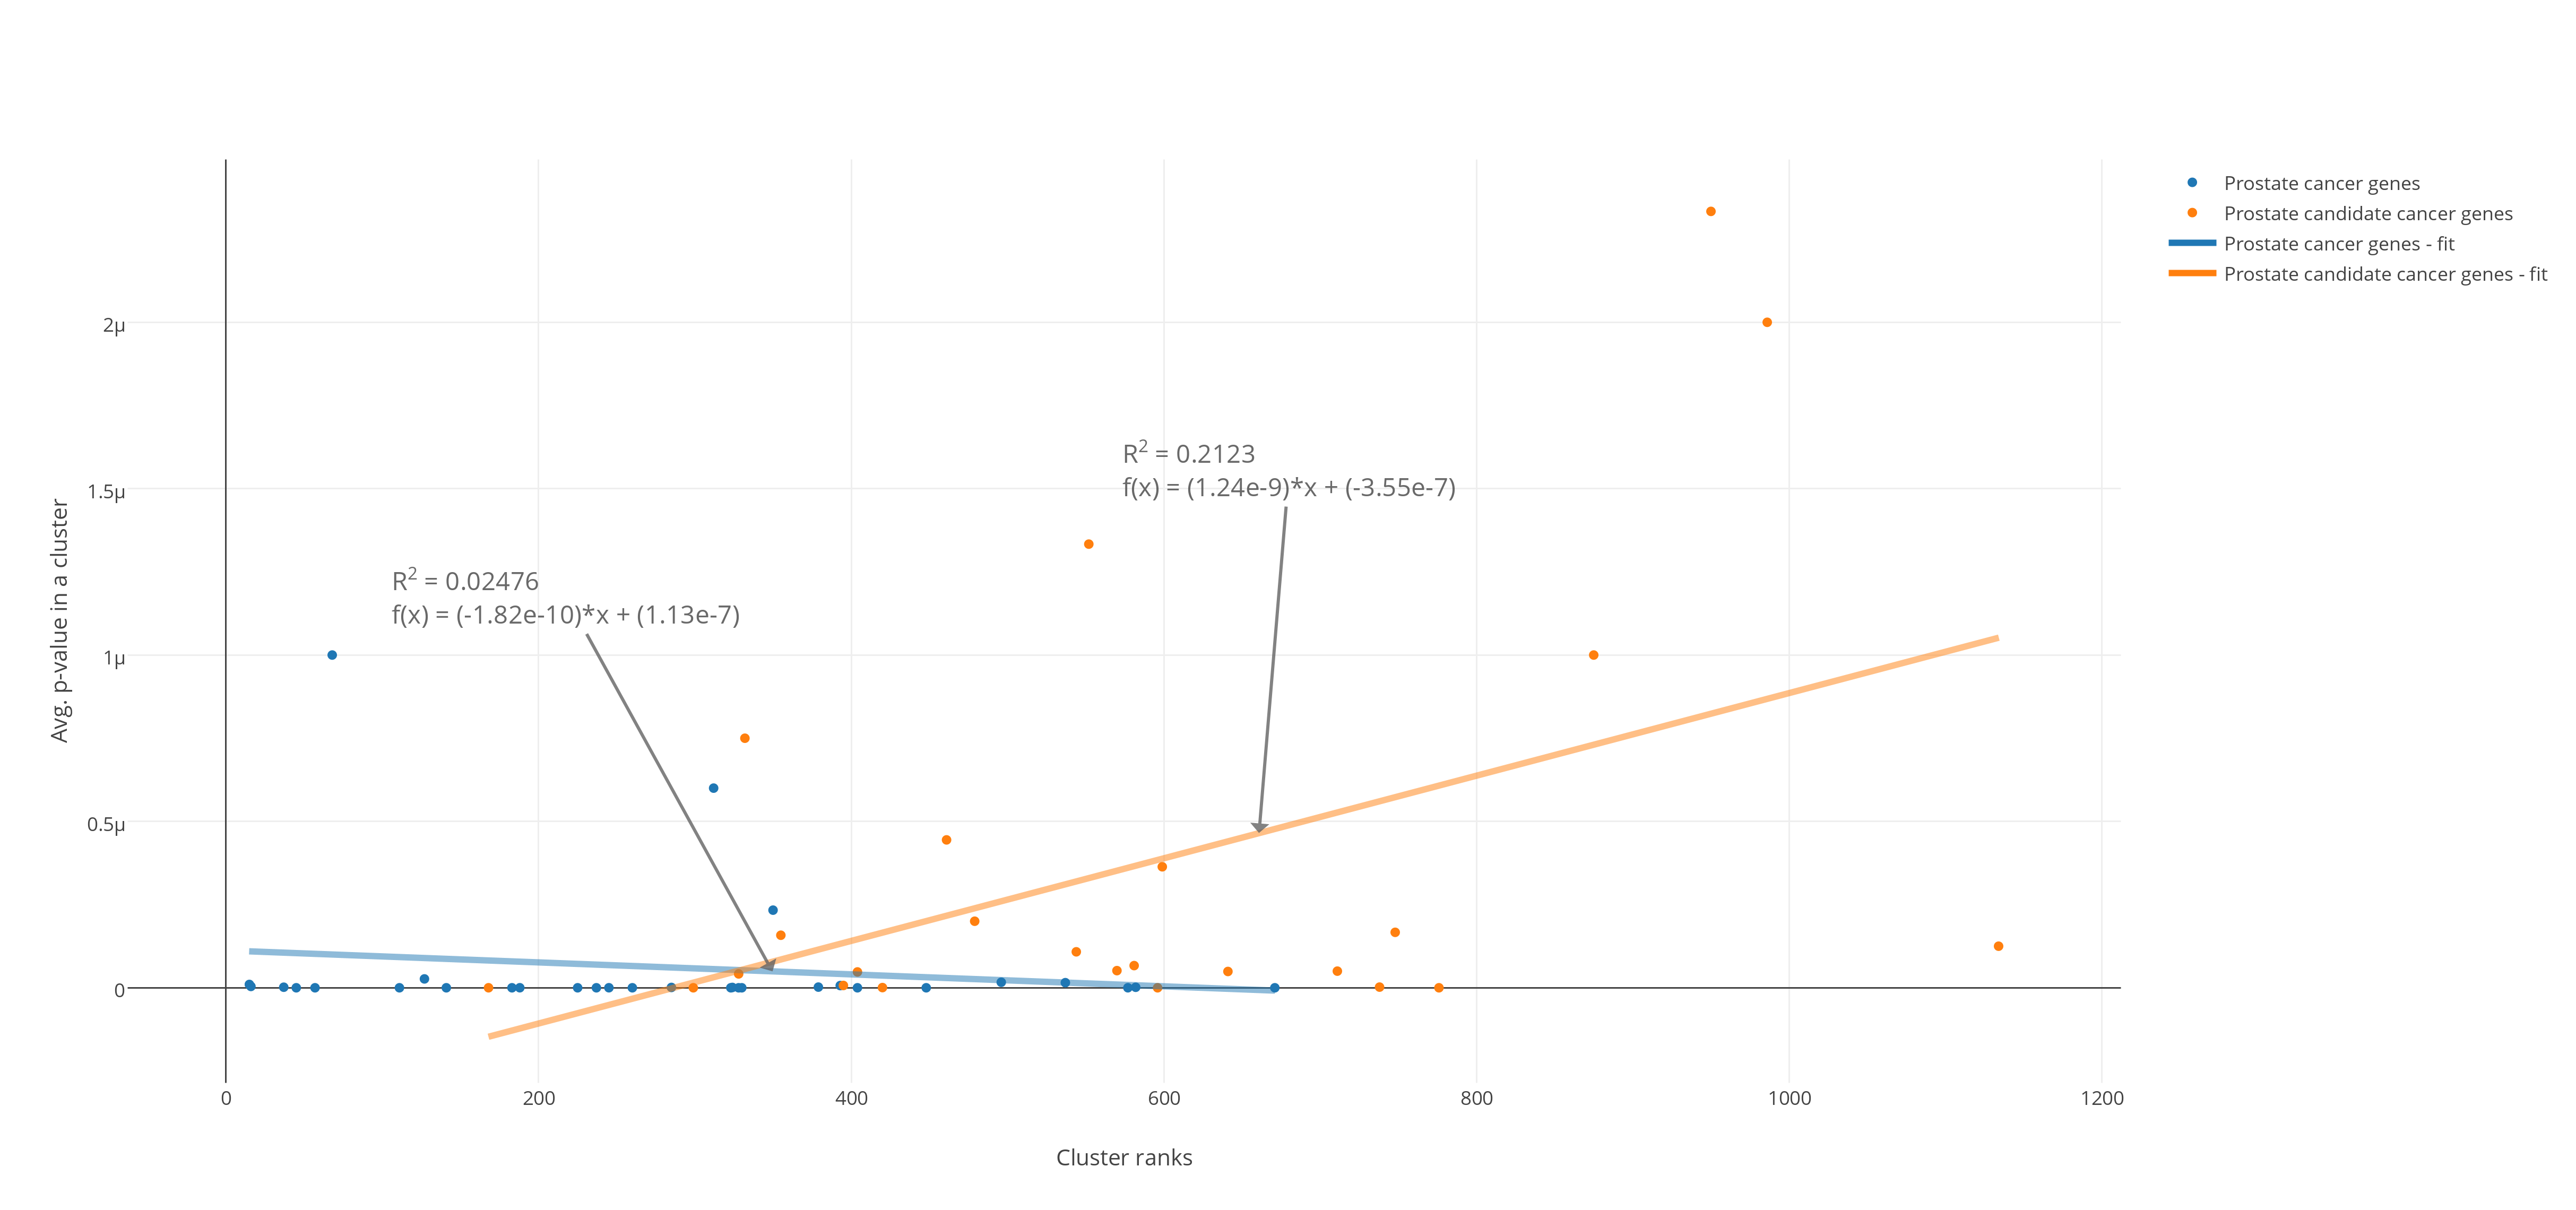
\includegraphics[scale=0.63]{prwp_exp_split}
    \caption{Average distribution of p-values in clusters ranked by PRWP.}
\end{sidewaysfigure}
\begin{sidewaysfigure}
    \label{fig:exp-iref-maa}
    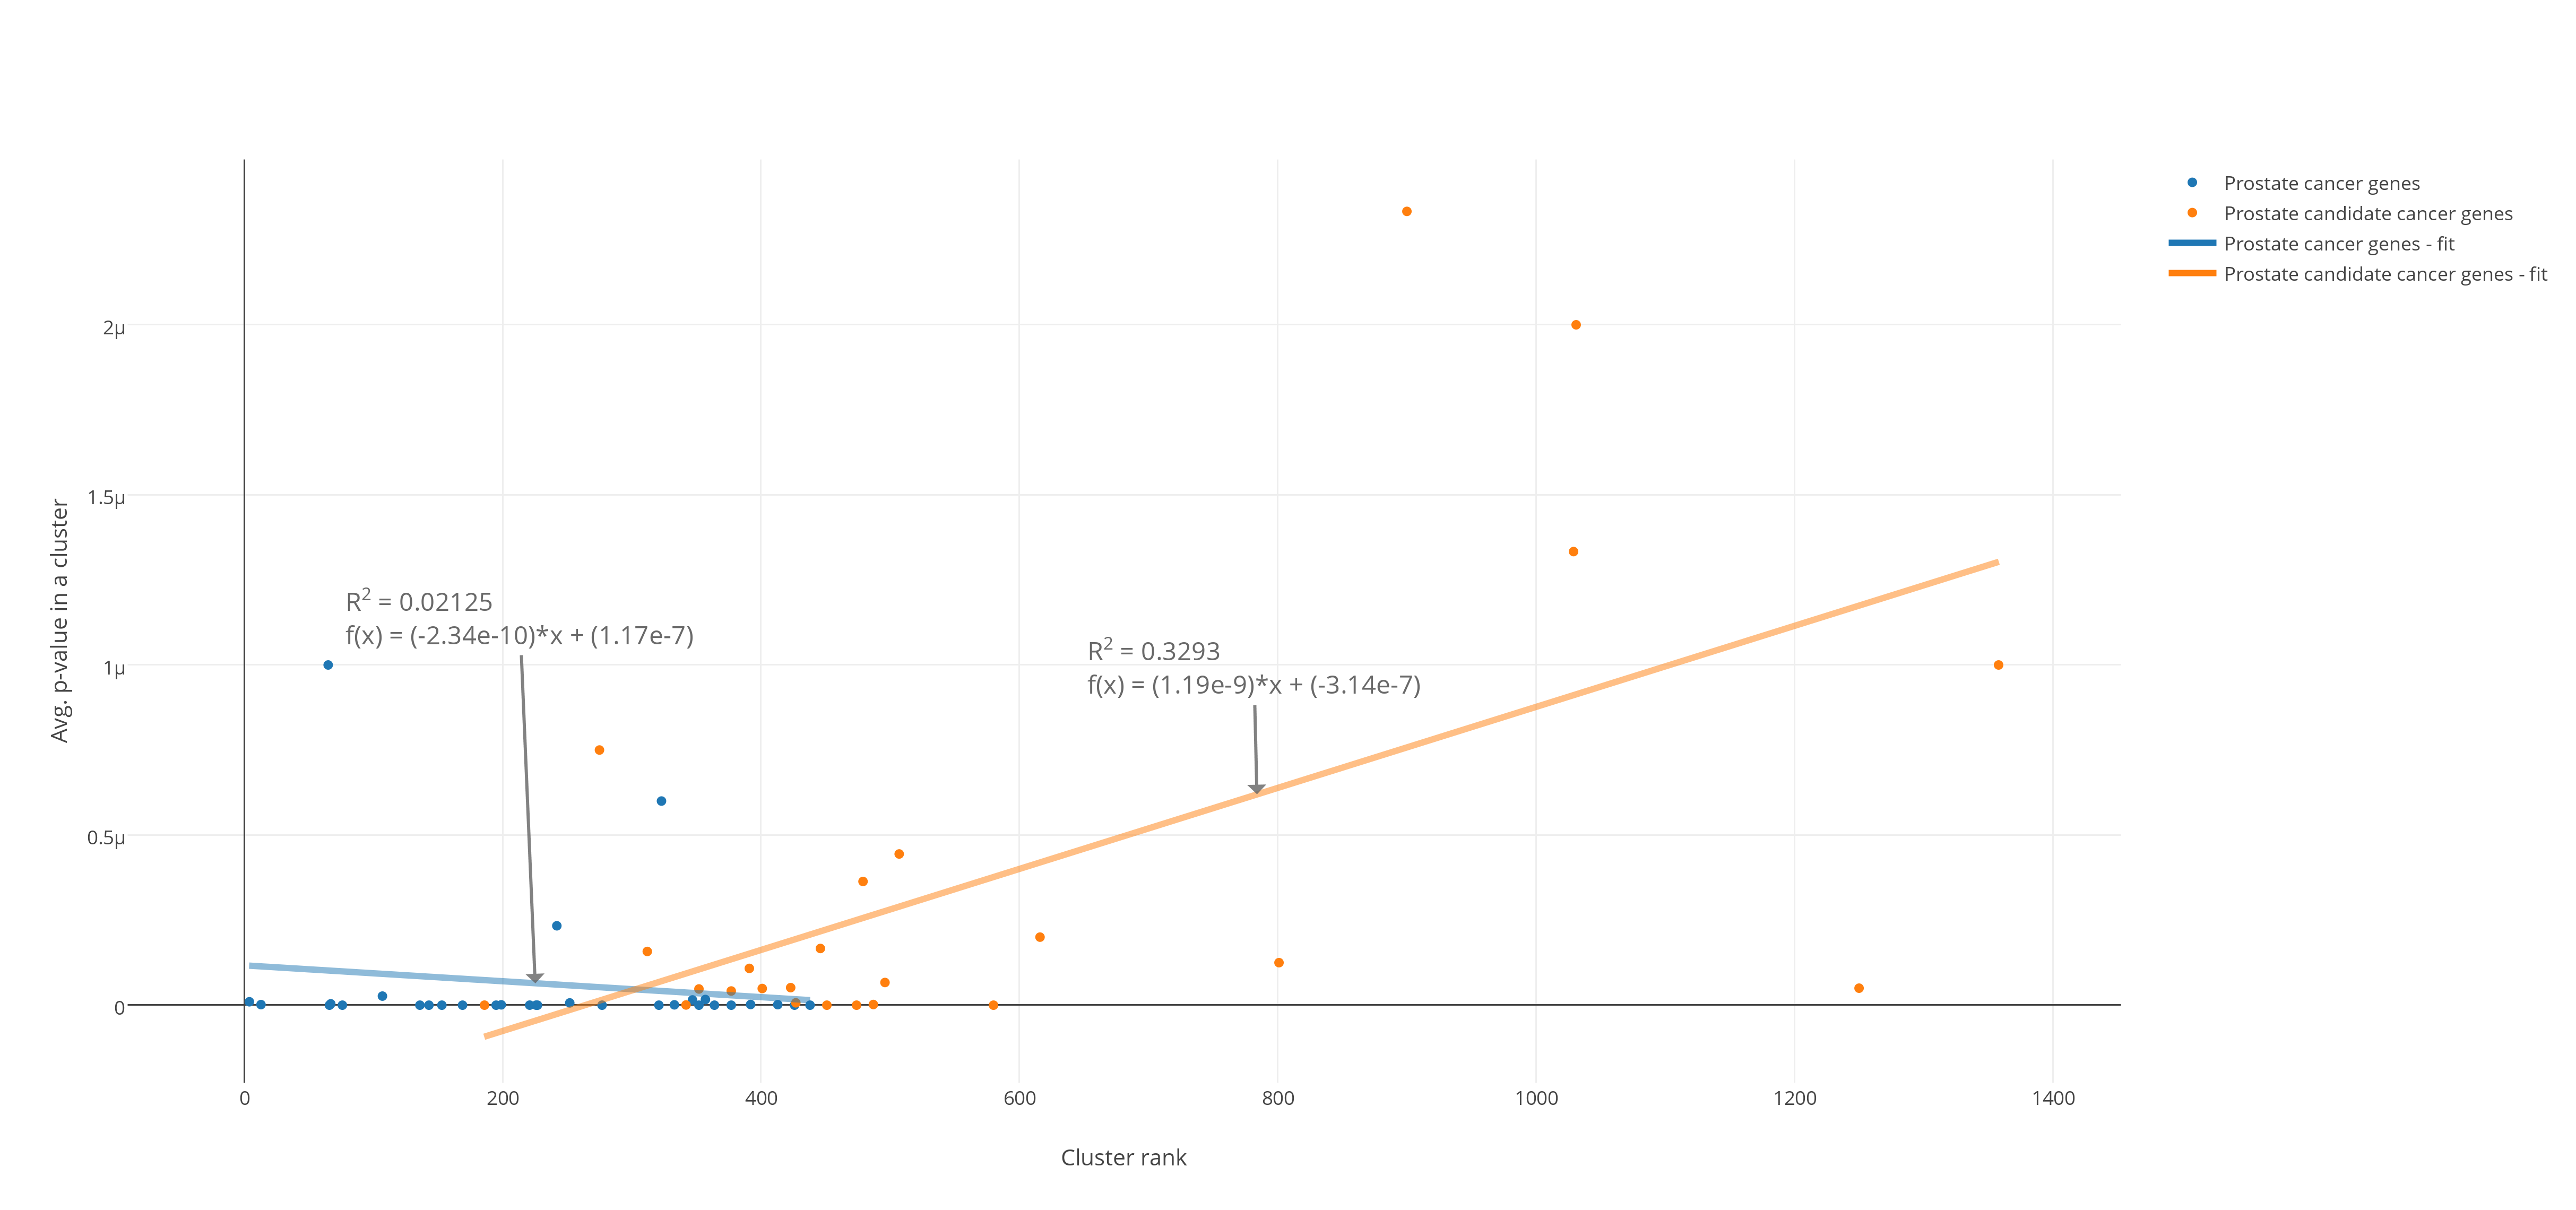
\includegraphics[scale=0.63]{maa_exp_split}
    \caption{Average distribution of p-values in clusters ranked by MAA.}
\end{sidewaysfigure}

All of the experimental genes are from experiments and are a result from
genome-wide association studies (GWAS). Each gene in this test data are scored
after p-values from "the most statistically significant SNP within the
block."\cite{distild} in experiments related to prostate cancer. The
\gls{jensen} database has experimental data from both the Catalogue of Somatic
Mutations in Cancer (COSMIC) and DistiLD, but for prostate cancer, only
experimental data from DistiLD was available.

The score for each cluster is calculated from the average p-value from each gene
in the cluster. In contrast to the previous plots, the trend required to
validate \gls{prwp} and \gls{maa} as cluster ranking algorithms for prioritizing
network biomarkers in prostate cancer, is an ascending trend in both genes with
and without prior scores, when ranking clusters from the topmost to the lowest
cluster. An ascending score for the genes with prior scores proves that the
highly ranked clusters have low p-values, which is proof of a low chance of the
null hypothesis being true. Here, the null hypothesis would be that a gene has
no relevance to prostate cancer. The \gls{golden} is based on \gls{dragon} and
DisGeNET scores. The DisGeNET scores are developed as a score based on the
supporting evidence for the context of a gene and a disease being
true\cite{disgenet}. Based on this fact, it is feasible if \gls{prwp} and
\gls{maa} would demonstrate the previously defined trend.

The experimental data has one of the same feats as the manually knowledge
curated data, it is very sparse. As with the previous plots, the genes with
prior scores in a cluster are colored blue, and the ones without prior scores as
orange.

\subsubsection{PRWP benchmarked by experimentally mined genes}
For \gls{prwp} (figure: \ref{fig:exp-iref-prwp}), there is a trend for descending
p-values for the genes with prior scores in a cluster and an ascending p-value
trend for the genes without prior scores in a cluster. For the genes without
prior scores, this is a feasible result in order to validate Ranklust as a tool
for prioritizing network biomarkers. For the genes with prior scores, there is
a single cluster that seems to be the cause of the descending trend but the
\gls{rsquared} value for the fit of the linear regression is not high.

\subsubsection{MAA benchmarked by experimentally mined genes}
For \gls{maa} (figure: \ref{fig:exp-iref-maa}), the trends are the same as with
\gls{prwp}, but the trends are more noticeable. For the genes with prior scores,
the descending p-value trend towards the lower ranked clusters are steeper than
the one in the plot for \gls{prwp}, but the \gls{rsquared} score is very low and
the as it is in the \gls{prwp} plot, it seems to be a single cluster that is
responsible for the descending trend in p-values.

\subsubsection{Conclusion of benchmarking through experimentally mined genes}
As with the manually knowledge curated genes, the experimental genes have
a small sampling size. Also, the trends that would discredit Ranklust's ability
to prioritize network biomarkers is not backed up by very high values of
confidence in terms of \gls{rsquared} values in the linear regression fits. In
this specific case of benchmarking Ranklust, it is a high probability that the
cause of the trend is an outlier in the plot.

\section{Comparison of PRWP and MAA to prostate cancer relevant genes}
Using \gls{prwp} and \gls{maa}, 6 final lists of prioritized network biomarkers
for prostate cancer will be presented. These 6 lists will be the result of
3 \gls{prwp} and 3 \gls{maa} ranked clusters from the whole iRefWeb filtered
network with gene names and the scored with the full \gls{golden}. Each of the
3 ranking results from both algorithms will use the same three sets of data,
namely movember, cosmica and lethal.

\subsection{Using Ranklust to rank the clusters of a network}
The exact workflow of using Ranklust to create the ranks that the test data is
compared to is exactly as explained earlier in both the methods chapter and the
workflow part of this results chapter.

\subsubsection{Step 1 - create the network and fill it with prior scores}
The network was downloaded from iRefWeb. This network consisted of protein
interactions to create an unweighted and undirected PPI network. These proteins
was then filtered with their corresponding gene names taken from HGNC. Most of
the proteins in the network did not have a corresponding gene name that HGNC
could match, so over half of the interactions was removed.

The \gls{golden} was created as explained earlier, with prostate cancer data
from DisGeNET and \gls{dragon}. The network was uploaded into Cytoscape and
populated with the prior scores. 

\subsubsection{Step 2 - Clustering the network}
The Markov Cluster algorithm, MCL, was used to cluster the iRefWeb network with
an inflation parameter of 1.8 and 200 iterations. This process took about 15
hours on the High-Performance Computing (HPC) instance Invitro at the University
of Oslo. It used a total of 64 cores, which averaged at a 90-95\% load for the
majority of the time the cluster algorithm ran.

\subsubsection{Step 3 - Ranking the clusters of the network}
\gls{prwp} and \gls{maa} was ran on the network, choosing only the priors in the
nodes given by the \gls{golden}. The alpha value for \gls{prwp} was set to 0.3
together with 30 max iterations.

\subsubsection{Step 4 - Exporting cluster ranks from Cytoscape and comparison with test data}
The node table with the results from \gls{prwp} and \gls{maa} was exported to
csv files, cleaned up with python scripts so it would form clusters containing
information about which genes was in which clusters, the rank of the cluster and
which genes in the cluster had a prior score or not.

The test data is in the form of a single column text file where each row
contains the name of a gene. By traversing the ranked list of clusters, four
categories were made from these test data genes. 

The first two was named "test biomarkers" and "test candidates". These two have
in common that they both list genes from the cluster in its column if it is
contained in the test data set of genes. The "test biomarkers" are genes that
both have a prior score and are contained in the test data set of genes. The
"test candidates" are also in the test data set of genes, but they do not have
prior scores.

The next two categories are "remaining biomarkers" and "remaining candidates".
These two categories have in common that neither of them will list genes that
was in the test data set of genes. The difference is that "remaining biomarkers"
have prior scores, and "remaining candidates" have no prior scores.

Each cluster had their genes split into these four categories, represented as
four columns in the next upcoming tables (tables: \ref{tab:prwp-movember}
\ref{tab:maa-movember}, \ref{tab:prwp-cosmic}, \ref{tab:maa-cosmic},
\ref{tab:prwp-lethal}, \ref{tab:maa-lethal}). The last column represents the
rank of the cluster from either \gls{prwp} or \gls{maa}, depending on the table.
From each of these tests, it is displayed the top 10 clusters, which had
a combined amount of genes in either the "test biomarkers" or the "test
candidates" column above 0.

\subsection{Prostate cancer genes manually curated from the movember group}
\begin{sidewaystable}
    \begin{tabular}{|l|l|l|l|l|}
        \hline
        \textbf{Rank}
        & \textbf{Test biomarkers}
        & \textbf{Test candidates}
        & \textbf{Remaining biomarkers}
        & \textbf{Remaining candidates} \\
        \hline
        13	& TNFRSF11B	& THBS1	& VEGFA	& - \\
        \hline
        19	& -	& F12	& MMP12	& - \\
        \hline
        25	& F2R	& -	& F2RL1	& PRTN3 \\
        \hline
        28	& -	& RRM2	& MAGEA3,MAGEA1	& DNM1L,PGAM5,SCG3 \\
        \hline
        29	& CEACAM1	& -	& -	& CLEC4M \\
        \hline
        31	& ALOX15B	& -	& -	& ERAL1 \\
        \hline
        46	& SMAD4	& -	& -	& ZMIZ1 \\
        \hline
        48	& STAT6	& -	& ACSL3,IFI16	& TRIM56,TMEM173,SLC39A14 \\
        \hline
        53	& RNASEL	& IQGAP1	& -	& GSPT1,NPHS2 \\
        \hline
        55	& DPP4	& -	& VIP,GHRH,ADCYAP1	& PYY,AVPR1A,GCG,GIP,TAC1,FAP,NPPB \\
        \hline
    \end{tabular}
    \caption{iRefWeb network ranked with PRWP and movember data - matched 254 
    test genes from movember data set out of 271 possible}
    \label{tab:prwp-movember}
\end{sidewaystable}

\begin{sidewaystable}
    \begin{tabular}{|l|l|l|l|l|}
        \hline
        \textbf{Rank}
        & \textbf{Test biomarkers}
        & \textbf{Test candidates}
        & \textbf{Remaining biomarkers}
        & \textbf{Remaining candidates} \\
        \hline
        8	& F2R	& -	& F2RL1	& PRTN3 \\
        \hline
        12	& TNFRSF11B	& THBS1	& VEGFA	& - \\
        \hline
        14	& STAT6	& -	& ACSL3,IFI16	& TRIM56,TMEM173,SLC39A14 \\
        \hline
        20	& -	& F12	& MMP12	& - \\
        \hline
        25	& SMAD4	& -	& -	& ZMIZ1 \\
        \hline
        26	& CD44	& -	& -	& SCYL3 \\
        \hline
        35	& CEACAM1	& -	& -	& CLEC4M \\
        \hline
        57	& BIRC5	& -	& -	& KCNJ6 \\
        \hline
        58	& ALOX15B	& -	& -	& ERAL1 \\
        \hline
        69	& -	& CRIP2	& UXT,RELA,ALPL	& NR1H4,NME5 \\
        \hline
    \end{tabular}
    \caption{iRefWeb network ranked with MAA and movember data - matched 172
    test genes from movember data set out of 271 possible}
    \label{tab:maa-movember}
\end{sidewaystable}

\subsection{Curated prostate cancer genes from the COSMIC database}
\begin{sidewaystable}
    \begin{tabular}{|l|l|l|l|l|}
        \hline
        \textbf{Rank}
        & \textbf{Test biomarkers}
        & \textbf{Test candidates}
        & \textbf{Remaining biomarkers}
        & \textbf{Remaining candidates} \\
        \hline
        6	& TNFAIP3	& -	& RNF14,TAGLN	& - \\
        \hline
        11	& BIRC3	& -	& -	& BIRC2 \\
        \hline
        12	& CXCR4	& -	& -	& CXCL14 \\
        \hline
        17	& -	& DAXX	& TGFBR3,ACVR2A	& TCTEX1D4 \\
        \hline
        18	& RHOA	& -	& AGER	& GMIP \\
        \hline
        24	& -	& ELN	& EFEMP2,SOD3,FBLN5	& - \\
        \hline
        37	& AR	& KMT2A	& MAK,TSPY1	& PKLR,HHAT \\
        \hline
        39	& TOP1	& -	& -	& RCVRN \\
        \hline
        44	& WIF1	& -	& -	& WNT11 \\
        \hline
        46	& SMAD4	& -	& -	& ZMIZ1 \\
        \hline
    \end{tabular}
    \caption{iRefWeb network ranked with PRWP and COSMIC data - matched 423 test
    genes from the COSMIC data set out of 580 possible}
    \label{tab:prwp-cosmic}
\end{sidewaystable}
prwp-cosmic: 423 out of 580

\begin{sidewaystable}
    \begin{tabular}{|l|l|l|l|l|}
        \hline
        \textbf{Rank}
        & \textbf{Test biomarkers}
        & \textbf{Test candidates}
        & \textbf{Remaining biomarkers}
        & \textbf{Remaining candidates} \\
        \hline
        1	& TNFAIP3	& -	& RNF14,TAGLN	& - \\
        \hline
        10	& RHOA	& -	& AGER	& GMIP \\
        \hline
        13	& AR	& KMT2A	& MAK,TSPY1	& PKLR,HHAT \\
        \hline
        14	& STAT6,ACSL3	& -	& IFI16	& TRIM56,TMEM173,SLC39A14 \\
        \hline
        15	& -	& DAXX	& TGFBR3,ACVR2A	& TCTEX1D4 \\
        \hline
        17	& BIRC3	& -	& -	& BIRC2 \\
        \hline
        19	& -	& SUFU	& PIAS1	& - \\
        \hline
        25	& SMAD4	& -	& -	& ZMIZ1 \\
        \hline
        29	& SET	& -	& -	& TAF1C \\
        \hline
        37	& TOP1	& -	& -	& RCVRN \\
        \hline
    \end{tabular}
    \caption{iRefWeb network ranked with MAA and COSMIC data - matched 277 test
    genes from the COSMIC data set out of 580 possible}
    \label{tab:maa-cosmic}
\end{sidewaystable}
maa-cosmic: 277 out of 580

\subsection{Proven prostate cancer genes that resulted in lethal outcome for the patient}
\begin{sidewaystable}
    \begin{tabular}{|l|l|l|l|l|}
        \hline
        \textbf{Rank}
        & \textbf{Test biomarkers}
        & \textbf{Test candidates}
        & \textbf{Remaining biomarkers}
        & \textbf{Remaining candidates} \\
        \hline
        25	& F2R	& -	& F2RL1	& PRTN3 \\
        \hline
        28	& -	& RRM2	& MAGEA3, MAGEA1	& DNM1L, PGAM5, SCG3 \\
        \hline
        31	& ALOX15B	& -	& -	& ERAL1 \\
        \hline
        55	& DPP4	& -	& VIP, GHRH, ADCYAP1	& PYY, AVPR1A, GCG, GIP, TAC1, FAP, NPPB \\
        \hline
        79	& BIRC5	& -	& -	& KCNJ6 \\
        \hline
        88	& SERPINA3	& -	& KLK4	& CTRC, GZMM, SGCD \\
        \hline
        91	& -	& CRIP2	& UXT, RELA, ALPL	& NR1H4, NME5 \\
        \hline
        92	& CCNB1	& UBE2C	& -	& UBE3D \\
        \hline
        114	& JAG1	& -	& -	& NEURL1, CD46 \\
        \hline
        120	& -	& CYB5A	& CYP17A1, CYP3A4, CYP3A5, CYP2E1	& CYP4F2, CYP4A11 \\
        \hline
    \end{tabular}
    \caption{iRefWeb network ranked with PRWP and lethal prostate cancer data
    - matched 99 test genes form the lethal prostate cancer data set out of 157
possible}
    \label{tab:prwp-lethal}
\end{sidewaystable}
prwp-lethal: 99 out of 157

\begin{sidewaystable}
    \begin{tabular}{|l|l|l|l|l|}
        \hline
        \textbf{Rank}
        & \textbf{Test biomarkers}
        & \textbf{Test candidates}
        & \textbf{Remaining biomarkers}
        & \textbf{Remaining candidates} \\
        \hline
        8	& F2R	& -	& F2RL1	& PRTN3 \\
        \hline
        57	& BIRC5	& -	& -	& KCNJ6 \\
        \hline
        58	& ALOX15B	& -	& -	& ERAL1 \\
        \hline
        69	& -	& CRIP2	& UXT,RELA,ALPL	& NR1H4,NME5 \\
        \hline
        79	& -	& RRM2	& MAGEA3,MAGEA1	& DNM1L,PGAM5,SCG3 \\
        \hline
        92	& CCNB1	& UBE2C	& -	& UBE3D \\
        \hline
        105	& JAG1	& -	& -	& NEURL1,CD46 \\
        \hline
        106	& DPP4	& -	& VIP,GHRH,ADCYAP1	& PYY,AVPR1A,GCG,GIP,TAC1,FAP,NPPB \\
        \hline
        109	& SERPINA3	& -	& KLK4	& CTRC,GZMM,SGCD \\
        \hline
        112	& -	& CYB5A	& CYP17A1,CYP3A4,CYP3A5,CYP2E1	& CYP4F2,CYP4A11 \\
        \hline
    \end{tabular}
    \caption{iRefWeb network ranked with MAA and lethal prostate cancer data
    - matched 66 test genes form the lethal prostate cancer data set out of 157
possible}
    \label{tab:maa-lethal}
\end{sidewaystable}
maa-lethal: 66 out of 157
